\chapter{Configuration Space Approximation \mbox{using} Active Learning} 
\label{chp:APD}

\section{Introduction}
\label{sec:2:intro}
Computing a high-quality configuration space representation is important for many applications, such as robotics~\cite{LPT:SpatialPlanning:1983}, physically-based simulation~\cite{Je:2012:PRP}, Minkowski sums~\cite{Varadhan:2006:TPA}, and offset computation~\cite{Choi:1997:CAD}. 
However, to compute an exact representation for a configuration space is time-consuming, because the complexity of this problem grows exponentially in the dimension of the configuration space. As a result, it remains a major challenge to represent and compute configuration spaces, especially for high dimensional ones.

\subsection{Main Results}
In this chapter, we present a novel algorithm to efficiently approximate a high-dimensional configuration space using machine learning techniques. The main idea is to generate samples in the configuration space and then use these samples to approximate the contact space $\Ccont$ by a separating surface that can correctly separate all the in-collision and collision-free samples. This separating surface is computed using SVM classification. Our method greatly reduces the required number of samples by leveraging incremental and active learning techniques. 
When the number of samples increases, the approximate contact space computed by our method can quickly converge to the exact contact space; we also provide bounds on the expected error in the approximate contact space. We evaluate performance of our algorithm on high-dimensional benchmarks.

Additionally, based on the approximate $\Ccont$ computed offline, we design a new method to efficiently approximate the penetration depth (PD) between two rigid objects. The penetration depth is the minimum amount of motion required to separate two intersecting objects. Our algorithm performs a nearest-neighbor query between a given query configuration and the precomputed $\Ccont$ approximation. Compared to prior techniques, our approach is more general and more reliable. Moreover, the runtime query only has a small overhead (a few milliseconds) and thus can be used for interactive applications. In practice, we are able to compute approximate PD with relative error less than 2-3\% by using a few thousand samples during the offline $\Ccont$ computation. We also use our PD algorithm to compute collision response between non-convex models in Box2D and Bullet physics engines. We observe more than an order of magnitude improvement in runtime performance over that of prior global PD algorithms.

\subsection{Organization}
The rest of this chapter is organized as follows. We survey related work on configuration space computation in Section~\ref{sec:2:related}. We introduce the notation and give an overview of our algorithm in Section~\ref{sec:2:overview}. The approach for approximating the configuration space using learning techniques is described in Section~\ref{sec:2:learning}. The approximate configuration space is then used for approximate PD computation, as discussed in Section~\ref{sec:2:approxPD}. We analyze the accuracy and convergence of our approximate PD algorithm in Section~\ref{sec:2:analysis}. The implementation details and experimental results are provided in Section~\ref{sec:2:result}.

\section{Related Work}
\label{sec:2:related}
\subsection{Configuration Space Construction}
There is extensive work on configuration space computation in robotics, geometric computing, and related areas.
Configuration space computation can be reduced to the problem of computing the arrangement of contact surfaces~\cite{Varadhan:2006:TPA}.
However, this approach is prone to problems involving accuracy and robustness. Moreover, the worst-case complexity of the entire arrangement can be as high as $\mathcal O(n^k)$, where $n$ is the number of contact surfaces in the arrangement and $k$ is the dimension of the configuration space~\cite{Goodman:Rourke:1997}. Some techniques for approximating the configuration space in lower dimensions are based on generating a discrete number of slices~\cite{Sacks:SCS:1997}. In this case, the configuration space is composed of many ruled surface patches, i.e., through each point on a surface patch, there exists a straight line that lies on the surface. These ruled surface patches are generated by different contact configurations between a vertex of an object and an edge from the other objects. When the object motion is limited to translation, the resulting configuration space is equivalent to the Minkowski sum between two objects~\cite{Leonidas:CCRS:1987,LPT:SpatialPlanning:1983}. Minkowski sum computation reduces the problem to computing either an arrangement or a union of a large set of convex primitives, which can be still very difficult in practice.

\subsection{PD computation}
PD computation has been studied extensively in computer graphics,
geometric modeling, haptics, and robotics. We give a brief
overview of exact and approximate computation algorithms.

Penetration depth is the minimum amount of motion transformation required to separate two intersecting objects. This transformation may correspond to only translation and the resulting PD is called the \emph{translational PD}; when this transformation corresponds to both translation and rotation, the resulting PD is called the \emph{generalized PD}.

For convex polytopes, exact translational PD can be computed using
the Minkowski sum~\cite{Gino:2001:GDC,Agarwal:2000:CPD,Kim:2002:DEEP}.
For non-convex objects, the PD can be computed using a combination of convex decomposition, pairwise Minkowski sums, and union computation~\cite{Kim:2002:FPD}. These algorithms are applicable to closed polyhedral shapes. The union computation has a high computational complexity. To address this issue, it is often approximated using rasterization hardware~\cite{Kim:2002:FPD}.

Most practical techniques for translational PD compute local PD
or some approximation of global PD. Local PD algorithms only take
into account local overlapping features (vertices, edges, and faces),
and compute a transformation to separate those
features~\cite{Guendelman:2003:NRB,Redon:2006:AFM,Lien:2009:ASM,Tang:2009:IHD,Tang:2012:CPF}. For example, local intersection volume and its derivative are used for volume-based repulsion in~\cite{Wang12}.
Distance fields are also used for local translational PD
computation~\cite{Heidelberger04} and can be computed in realtime using GPUs.
Point-based Minkowski
sum approximation~\cite{Lien:2008:CMS} can also compute global translational PDs.

Exact generalized PD can be computed by constructing the
exact contact space and then searching the contact space for the
closest point to a given query~\cite{Zhang:2007:GPD}. However,
due to high time and storage complexity, most
generalized PD algorithms use optimization-based
techniques~\cite{Nawratil:2009:GPD,Zhang:2007:AFP,Je:2012:PRP} and compute a locally
optimal solution based on local approximation of the contact space.

Machine learning techniques have been used for collision detection~\cite{Doshi:2007:ISRR,Pan:2011:ISRR}. However, these techniques cannot be used for PD computation directly. One reason is that in pratice, checking for collisions is much easier than computing the PD between overlapping objects.

\section{Background and Overview}
\label{sec:2:overview}
In this section, we introduce our notation and give an overview of our approach. We first present PD formulation in terms of configuration space and then describe our approach to computing approximate $\Ccont$ using learning techniques, which is then used for efficient computation of approximate PD.

\subsection{Contact Space and PD Formulation}
\subsubsection{Contact Space}
As we mentioned in Section~\ref{chp:intro}, the contact space $\Ccont$ is the boundary of $\Cobs$ and is denoted as $\Ccont =\partial \Cobs$. We use the notation $c(\q) \in \{-1,+1\}$ to denote the collision state of a configuration $\q$, i.e., $c(\q)=+1$ if $\q \in \Cobs$ and $c(\q)=-1$ if $\q \in \Cfree$.

\subsubsection{PD Formulation}
\label{sec:2:overview:pdformulation}
We define global penetration depth as the minimum motion or transformation required to separate two intersecting objects $A$ and $B$~\cite{Agarwal:2000:CPD,Kim:2002:DEEP}:

\begin{align}
\label{eq:2:PDgdef} \text{PD}(A(\qa), B) = \min_{\q \in
\Ccont} \dist(\qa, \q),
\end{align}
where $\qa$ is an in-collision configuration and $\q$ is a
configuration that lies in the contact space $\Ccont$.
We use the notation $\dist(\cdot, \cdot)$ to represent the distance between two configurations,
which may correspond to any metric defined on the $\Cspace$. The
contact point or configuration for which PD$(A, B)$ attains its
minimal value is denoted as $\qc = \argmin_{\q
\in \Ccont} \dist(\qa, \q)$.

In this chapter, we focus on the translational and rotational motion. Different types of motion require different $\dist(\cdot,\cdot)$ metrics.
For translational PD ($\PDt$), the commonly used $\dist(\cdot, \cdot)$ is the standard Euclidean distance metric between dim-3 vectors corresponding to the configurations. Many distance metrics have been proposed for generalized PD ($\PDg$) computation, including weighted Euclidean
distance~\cite{Wang:CBO:2012}, object norm~\cite{Je:2012:PRP}, and displacement distance metric~\cite{Zhang:2007:AFP}. We use the displacement distance metric in our algorithm, which is defined as:
\begin{align}
\label{eq:PDgmetric}
\dist(\mathbf q_i, \mathbf q_j) = \mu_1 q_1^2 + \mu_2 q_2^2 + \mu_3 q_3^2 + q_4^2 + q_5^2 + q_6^2,
\end{align}
where $(q_1, q_2, q_3)$ and $(q_4, q_5, q_6)$ measure the relative rotation and the relative translation between two configurations $\mathbf q_i$ and $\mathbf q_j$, respectively. $(q_0, q_1, q_2, q_3)$ corresponds to the relative quaternion between these two configurations, where $q_0=(1- q_1^2-q_2^2-q_3^2)^{1/2}$. $\mu_i$ is the weight on the rotational component and is computed as~\cite{Zhang:2007:AFP}:
\begin{align}
\mu_1 = \frac{4}{\vol}I_{xx}, \ \ \  \mu_2 = \frac{4}{\vol}I_{yy}, \ \ \  \mu_3 = \frac{4}{\vol}I_{zz},
\end{align}
where $\diag(I_{xx}, I_{yy}, I_{zz})$ represents the diagonal of the inertia matrix of the object $A$ and $\vol$ is the volume of the object $A$. 


\subsection{Approximate $\Ccont$ Computation}
To construct a representation of the configuration space, we use an offline learning algorithm as shown in the left box in Figure~\ref{fig:2:pipeline}. We first generate a small set of uniform samples in a subspace of $\Cspace$ for two given objects. Next, we justify whether these configurations lie in $\Cfree$ or in $\Cobs$ by performing exact collision checking between the two objects. Given the collision states ($-1$ or $+1$) of all configuration samples, a coarse approximation to the contact space, $\LCSa$ (Figure~\ref{fig:2:pipeline}(b)), is computed using classifiers, where $\LCS$ stands for \emph{Learned Contact Space}. Next, we select new samples in $\Cspace$ to further improve the accuracy of the initial representation $\LCSa$ using active learning. During active learning, we either select samples that are far away from prior samples (\emph{exploration}) (Figure~\ref{fig:2:pipeline}(c)) or samples that are near $\LCSa$ (\emph{exploitation}) (Figure~\ref{fig:2:pipeline}(d)).
After the new samples are generated, we compute an updated
approximation $\LCSb$ (Figure~\ref{fig:2:pipeline}(e)) based on incremental
machine learning techniques. We repeat this process, generating a sequence of approximate representations
$\LCSa$, $\LCSb$, ..., with increasing accuracy. This iterative process is repeated until the
collision states of all the new samples can be correctly
predicted by the current approximation. The final result $\LCS$
(Figure~\ref{fig:2:pipeline}(f)) corresponds to a smooth surface approximation of the contact space.

\subsection{Approximate PD Computation}
Given the approximate representation of the contact space, we can
then compute the approximate global PD by performing a nearest-neighbor query in the $\Ccont$.
The definition of approximate penetration depth is analogous to the exact penetration depth in Equation~\ref{eq:2:PDgdef}:

\begin{align}
\label{eq:2:PDsdef} \overline{\text{PD}}(A(\qa), B) = \min_{\q \in \LCS}\dist(\qa, \q),
\end{align}

Thus, the accuracy of $\overline{\text{PD}}$ is determined by the accuracy of $\LCS$.

As shown in Figure~\ref{fig:2:pipeline}(g), given a relative configuration $\qa$, we perform
a nearest-neighbor search to find a configuration that is closest to the decision boundary $\LCS$ and then project it
onto $\LCS$. We denote this projection result as $\qc$.
Finally, the distance between $\qa$ and $\qc$ is computed using an appropriate distance metric $\dist(\cdot, \cdot)$ and the result is an approximation to the exact PD value.


\begin{figure}[htb]
  \centering
  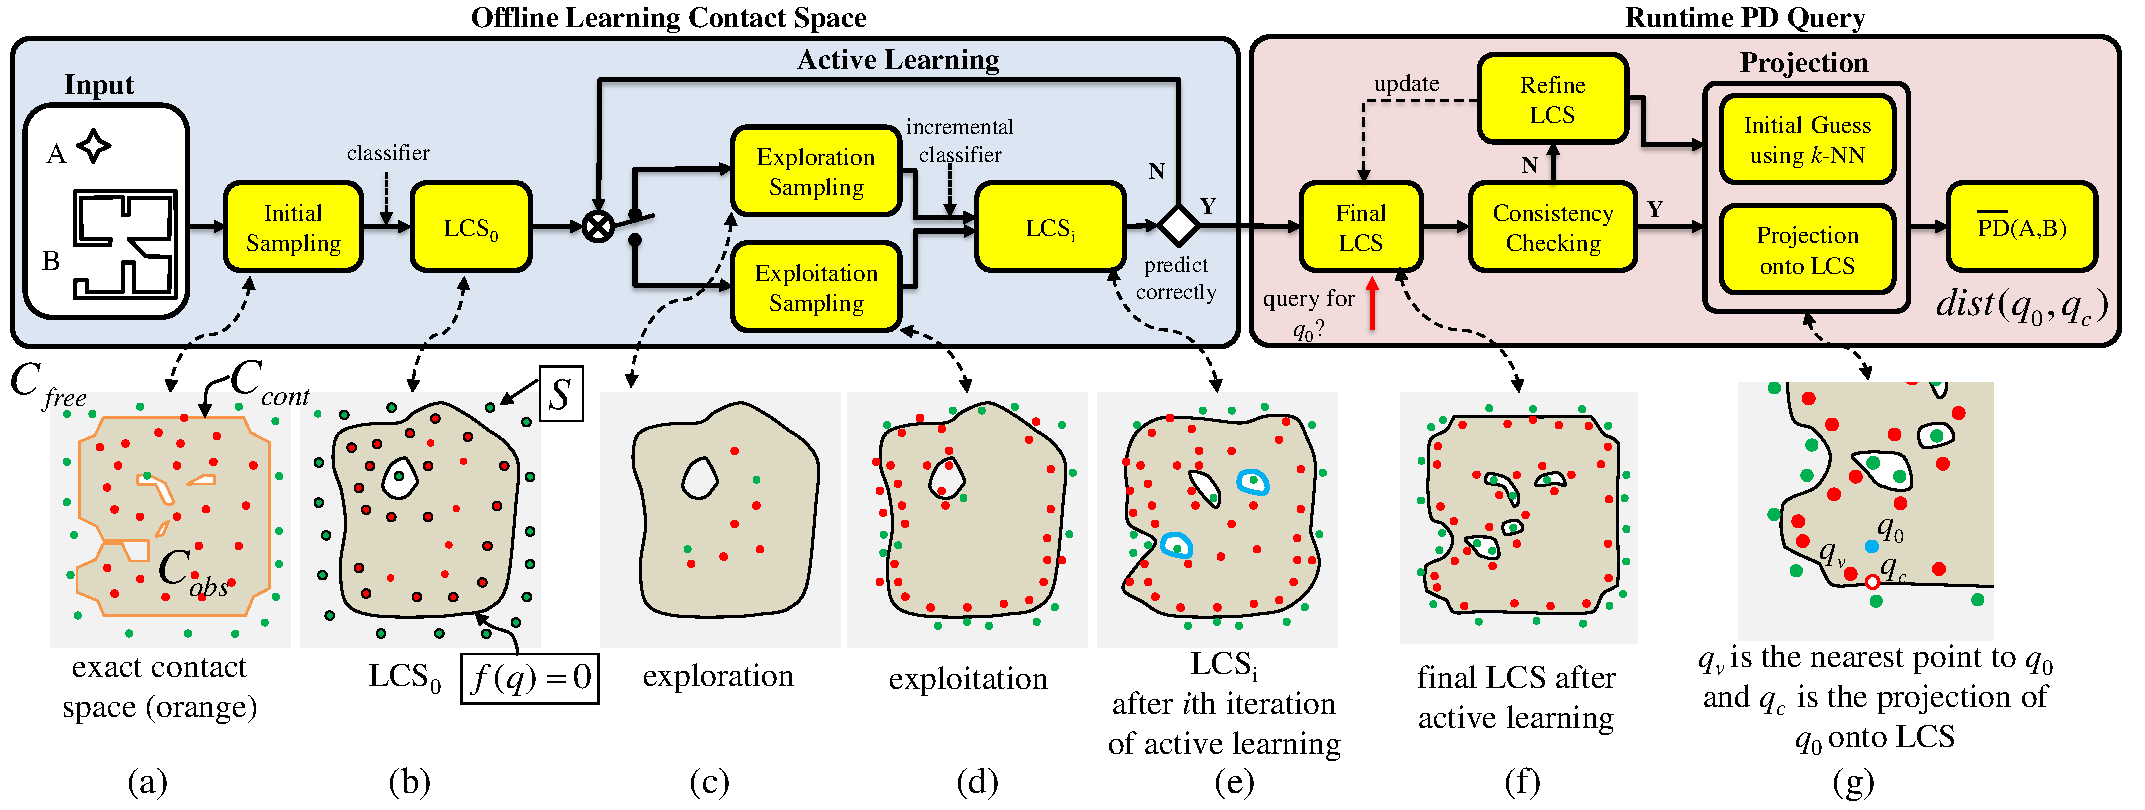
\includegraphics[width=\linewidth]{figs/2/pipeline.pdf}
  \caption[Offline computation pipeline for $\Ccont$ approximation and the runtime algorithm to compute the PD for a given query configuration]{This figure shows the offline computation pipeline for $\Ccont$ approximation and the runtime algorithm to compute the PD for a given query configuration. The different approximations of $\LCS$ are shown below the corresponding stages. We use green points to indicate collision-free configuration samples and red points to indicate in-collision samples.}
  \label{fig:2:pipeline}
\end{figure}

\section{Contact Space Construction via Machine Learning}
\label{sec:2:learning}
We now present our algorithm for the offline learning of the contact space and the computation of $\LCS$. Different stages of this algorithm
are shown in Figure~\ref{fig:2:pipeline}.

\subsection{Initial Sampling}
\label{sec:2:offline:uniform}

We perform uniform sampling in $\Cspace$ to obtain a set of configuration points. Rather than sampling the entire $\Cspace$,
we generate samples in a subspace that contains $\Ccont$. Given two objects $A$ and $B$, the contact space $\Ccont$ is contained in the in-collision space of their bounding volumes $BV(A)$ and $BV(B)$. We choose to use
axis-aligned bounding boxes (AABB) as the underlying BVs for $\PDt$
computation, due to their translational invariance in $\Rsqr$
and $\Rcubic$. Similarly, we use spheres as the underlying BVs for $\PDg$
computation due to their translational and rotational invariance in
$\SEsqr$ and $\SEcubic$.

The uniform sampling in the in-collision space of $BV(A)$ and $BV(B)$ can be implemented as follows. 
For $\PDt$ computation, the in-collision space of $BV(A)$ and $BV(B)$ is a box region, since it is the Minkowski sum of two axis-aligned bounding boxes. Samples uniformly distributed within this box region are guaranteed to cover the entire $\Ccont$.

For $\PDg$ computation, suppose that the given two bounding spheres are $(\mathbf c_A, r_A)$ and
$(\mathbf c_B, r_B)$, where $\mathbf c$ denotes a sphere center and $r$ denotes a sphere radius. We generate configuration samples for which these two bounding spheres are in collision. These samples correspond to all $(\mathbf R, \mathbf T)$ satisfying $\|\mathbf R \mathbf c_B + \mathbf T - \mathbf c_A\|_2 \leq r_A + r_B$, where $\mathbf R$ and $\mathbf T$ are the rotational and translational components of a configuration $\mathbf q$. We first generate one sample for the rotational component $\mathbf R$. For 2D rotation, we simply perform the uniform sampling within $[0, 2\pi]$; for 3D rotation, we use the method presented in~\cite{Shoemake:1992:URR} to sample $\SOcubic$ uniformly. After a random $\mathbf R$ is computed, the translational component $\mathbf T$ is uniformly distributed within a sphere $\|\mathbf T - (\mathbf c_A - \mathbf R \mathbf c_B)\| \leq r_A + r_B$; the uniform sampling within a sphere can be implemented using the well-known inverse-transform method. By repeating the above process many times, we can generate a sequence of $(\mathbf R, \mathbf T)$ uniformly distributed within the contact space of $A$ and $B$'s bounding spheres.

\subsection{Compute $\LCSa$} \label{sec:2:offline:model}
Given a set of $k$ samples from
$\Cobs(BV(A),BV(B))$, we perform exact collision queries between $A$ and $B$ to
check whether these samples are within in-collision space or not. Note that performing Boolean or discrete collision queries between complex models is a much easier problem compared to PD computation, as shown in Section~\ref{sec:2:analysis:timespacecomplexity}.
Our goal is to learn an approximate representation $\LCSa$ from these
configurations. In particular, $\LCSa$ corresponds to a decision function
$f(\q)=0$ that is fully determined by a set of configurations $\SV$
in $\Cspace$. We refer to $f(\q)$ as the \emph{classifier} and use it to
predict whether a given configuration $\q$ is collision-free
($f(\q)<0$) or in-collision ($f(\q)>0$). $\SV$ corresponds to the \emph{support vectors}, which are a
small subset of configuration samples used in learning.
Intuitively, $\SV$ are the samples that are closest to $\Ccont$.

Other options exist for computing the approximate contact space.
One alternative is to use surface fitting techniques to approximate the contact space by an implicit function, but this becomes more challenging for high-dimensional configuration spaces (e.g., 6-DOF $\Cspace$). Another possibility is to use regression-based learning techniques to approximate the contact space. However, such techniques typically require an improved or continuous approximation of PD values at these samples, which is much harder to compute compared to discrete collision queries.

\subsubsection{Nonlinear Classifier based on SVM}
\label{sec:2:offline:svm}
We use the SVM classifier~\cite{Vapnik:1995:NSL} to learn $\LCSa$ from
the initial sampling of $k$ configurations.
A SVM generates a decision function that is a smooth nonlinear surface. We use the
hard-margin SVM, as the underlying samples can
always be separated into collision-free and in-collision spaces. Intuitively, a SVM 
uses a function to map the given samples $\{\mathbf q_i\}$ from the \emph{input space} into a higher (possibly infinite) dimensional \emph{feature space}.
A SVM computes a linear
separating hyperplane characterized by parameters $\mathbf w$ and $b$. The hyperplane's maximal margin
is in the higher dimensional feature space. The hyperplane corresponds to a nonlinear separating surface in the input space. The $\mathbf w$ is the normal vector to the hyperplane, and the
parameter $b$ determines the offset of the hyperplane from the
origin along the normal vector. In the feature space, the distance between a hyperplane and the closest sample point is
called the `margin', and the optimal separating hyperplane should maximize this distance.
The maximal margin can be achieved by solving the following
optimization problem:
\begin{align}
\label{eq:2:svm1}
& \underset{\mathbf w, b}{\text{min}} & & \frac{1}{2}\|\mathbf w\|^2 & &  \\
& \text{subject to} & & c_i (\mathbf w \cdot \phi(\mathbf q_i) + b)
\geq 1, & & 1 \leq i \leq k. \notag
\end{align}
where $c_i \in \{-1,+1\}$ is the collision state of each sample ${\mathbf q_i}$.

Let $K(\mathbf q_i, \mathbf q_j) = \phi(\mathbf q_i)^T
\phi(\mathbf q_j)$ represent the kernel function (i.e., a function
used to calculate inner products in the feature space). The distance
between two points $\phi(\mathbf q_i)$ and $\phi(\mathbf q_j)$ in
the feature space can be computed as:
\begin{flalign}
\label{eq:2:svmdist}
&\|\phi(\mathbf q_i)-\phi(\mathbf q_j)\| \nonumber\\
&= \sqrt{K(\mathbf q_i, \mathbf q_i) + K(\mathbf q_j, \mathbf q_j)
- 2 K(\mathbf q_i, \mathbf q_j)}.
\end{flalign}
In our algorithm, we use the radial basis function (RBF) as the kernel:
$K(\mathbf q_i, \mathbf q_j) = \exp(-\gamma \|\mathbf q_i - \mathbf
q_j\|^2)$, where $\gamma$ is a positive parameter. In practice, we use $\gamma = 20$. We use the RBF kernel because it maintains the distance ranking
in both the input space and the feature space due to the fact that $\|\phi(\mathbf q_i) - \phi(\mathbf q_j)\|_2^2 = 2 - 2 \cdot \exp(-\gamma \|\mathbf q_i - \mathbf q_j\|_2^2)$.

The solution of Equation~\ref{eq:2:svm1} is a nonlinear surface in the
input space (and a hyperplane in the feature space) that separates
collision-free and in-collision configurations. This solution can be
formulated as:
\begin{align}
\label{eq:2:svmf} f(\mathbf q) = \mathbf w^* \cdot \phi(\mathbf q) +
b^* = \sum_{i=1}^k \alpha_i c_i K(\mathbf q_i, \mathbf q) + b^*,
\end{align}
where $\mathbf w^*$ and $b^*$ are the solutions of
Equation~\ref{eq:2:svm1} and $\alpha_i \geq 0$. 
The vectors $\mathbf q_i$ corresponding to the non-zero $\alpha_i$ are called
the \emph{support vectors}, which we denote as $\SV$. Intuitively, the support vectors
are those samples closest to the separating hyperplane
$f(\mathbf q) = 0$, as shown by the larger red and green points in
Figures~\ref{fig:2:pipeline}(b) and ~\ref{fig:2:pipeline}(g).
Thus, $\LCSa$ consists of an implicit function
$f_{\LCSa}(\q) = f(\q)$ and a set of samples
$S_{\LCSa}=S$ (i.e., the support vectors), which
are used to approximate the exact contact space.


\subsection{Refine $\LCSa$ using Active Learning}
\label{sec:2:offline:activelearning}
We refine $\LCSa$ using active learning. The
goal is to actively select new samples so that a better
approximate contact space representation, $\LCSb$, can be obtained by incorporating
these samples into $\LCSa$. We use a
combination of exploration and exploitation~\cite{Huang:2010:ALQ}.
The idea is to determine whether to explore
or to exploit by flipping a biased coin with a certain probability for landing on heads
(initially $0.5$). If the result is a head, we apply exploration;
if it is a tail, we apply exploitation. The probability of landing on heads is adjusted
according to the fraction of exploration samples' collision
states that are correctly predicted by the current $\LCSi$. The new
samples are used to update $\LCSa$ and generate a new approximation
$\LCSb$ (or refine from $\LCSi$ to $\LCSiplus$). We repeat the active
learning step until all the new samples can either be correctly
predicted by the current $\LCSi$, or the final result (represented
as $\LCS$) has sufficient accuracy to approximate $\Ccont$. Later in Section~\ref{sec:2:analysis}, we show that active learning results in improved convergence compared to uniform or random sampling schemes.


\subsubsection{Exploration}
$\LCSa$ may miss some holes or components corresponding to collision-free regions, if no initial samples were generated inside those regions. As a result, there may be some portions that $\LCSa$ may incorrectly classify, as shown in Figure~\ref{fig:2:pipeline}(c). In this case,
exploration refers to generating samples far away from prior
samples in order to explore the regions not well-sampled by the
current $\LCSi$. In our algorithm, we use random sampling to
explore these new regions (Figure~\ref{fig:2:pipeline}(c)). As
shown in Figure~\ref{fig:2:pipeline}(e), two new collision-free
regions (marked as blue curves) are found using exploration. After
each exploration sampling step, we compute the fraction of the new
samples that are not correctly predicted by $\LCSi$ to dertermine whether the exploration improves $\LCSiplus$.
If this cutoff fraction is large (e.g., $0.3$), then we increase the probability for exploration; otherwise we
decrease it.


\subsubsection{Exploitation}
Exploitation refers to generating samples near the decision
function of a given approximation $\LCSi$.

For exploitation, we use a simple method based on the \emph{maximal margin} property
of SVMs. The maximal margin
property~\cite{Vapnik:1995:NSL} states that in the feature space, the decision function
will have the same distance to support vectors with different
labels (i.e., collision-free or in-collision). In order to obtain a sample near the
decision function $f_{\LCSa} = 0$, we first choose a pair of support
vectors that are close to each other, but have opposite labels.
Based on the maximal margin property, the midpoint of the two
supporting vectors lies on or near the decision function.
\begin{figure}[htb]
  \centering
  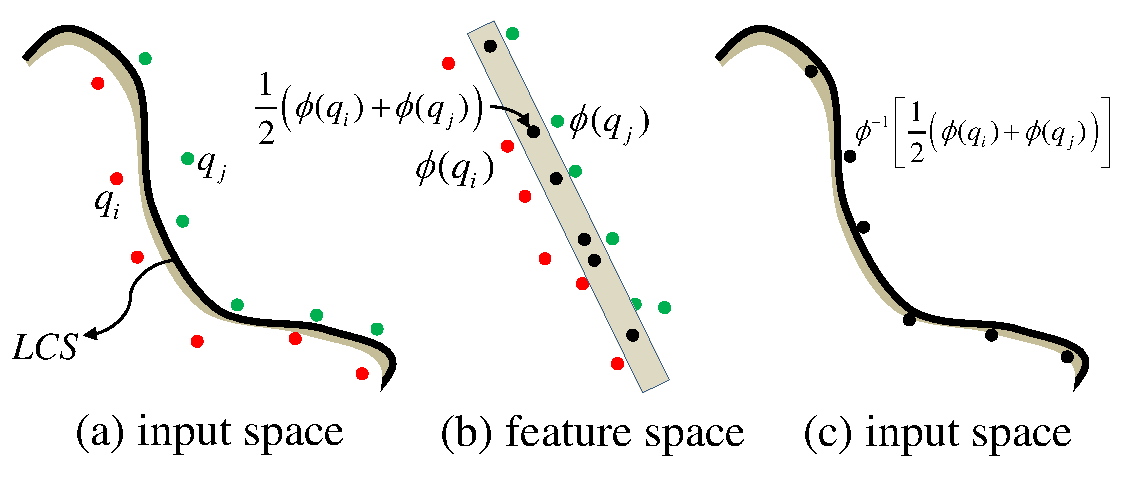
\includegraphics[width=0.6\linewidth]{figs/2/interpolation.pdf}
  \caption[Exploitation in SVMs]{Exploitation in SVMs:
  (a) support vectors are on different sides of the decision function ($\mathbf q_i$ and $\mathbf q_j$) in the input space;
  (b) their midpoints (black points) are computed in the feature space;
  (c) the pre-images of the midpoints lie near the decision function and can be used for exploitation.}
  \label{fig:2:interpolation}
\end{figure}
For nonlinear SVMs, the closest point and interpolation computations are
performed in the feature space. As shown in
Figure~\ref{fig:2:interpolation}, we first use the distance metric
mentioned in Equation~\ref{eq:2:svmdist} to find a pair of
supporting vectors $\mathbf q_i$ and $\mathbf q_j$. Next, we
compute their midpoint $\frac{1}{2}(\phi(\mathbf q_i) +
\phi(\mathbf q_j))$ (shown as black points in Figure~\ref{fig:2:interpolation}(b)). However, since the resulting midpoint may not have a pre-image in the input space, we search the input
space for a point $\q$ whose image $\phi(\q)$ in
feature space is closest to $\frac{1}{2}(\phi(\mathbf q_i) +
\phi(\mathbf q_j))$:
\begin{equation}
\begin{aligned}
\label{eq:2:preimage}
& \ \underset{\mathbf q}{\text{min}} & & \|\frac{1}{2}(\phi(\mathbf q_i) + \phi(\mathbf q_j)) - \phi(\mathbf q)\|_2 & \\
\Leftrightarrow & \ \underset{\mathbf q}{\text{max}} & & K(\mathbf q, \mathbf q_i) + K(\mathbf q, \mathbf q_j). &
\end{aligned}
\end{equation}
The solution is found using an optimization solver, in which the midpoint $\frac{\mathbf q_i +
\mathbf q_j}{2}$ in the input space is used as the initial guess. In our
benchmarks, this optimization solver tends to converge quickly
(in less than $10$ iterations).


\subsection{Incremental Learning}
\label{sec:2:incremental_learning}
Instead of computing a new decision function
from scratch using all the previous samples, we apply incremental
learning techniques to efficiently compute $\LCSiplus$ from
$\LCSi$. Incremental learning utilizes a small set
of new samples to update $\LCSi$. The decision function of $\LCSi$
serves as the initial guess for generating $\LCSiplus$. The incremental SVM~\cite{Karasuyama:2009:MID} can update
the current result generated using SVMs; the key is to retain the optimality condition of Equation~\ref{eq:2:svm1} (i.e., the Kuhn-Tucker condition) on all prior samples while adding new samples. This is achieved by adjusting the coefficients $\alpha_i$ and $b$ in Equation~\ref{eq:2:svmf} and by adjusting support vector set $\SV$. The coefficient adjustment and the support vector changes are guided by the gradient of the objective function in Equation~\ref{eq:2:svmf}.

\subsection{Terminating Active Learning}
Active learning terminates when either of these conditions has been satisfied:
\begin{enumerate}
    \item The collision states of all the new samples generated during
exploration and exploitation can be correctly predicted by the
current approximation $\LCSi$.
    \item The total number of samples used in active learning iterations is more than a user-specified threshold.
   \end{enumerate}
The first condition guarantees that all the configurations used for learning $\LCS$ are consistent (i.e., they can be correctly predicted by $\LCS$). This implies that the current $\LCS$ is a close approximation of the underlying contact space.
The second condition controls the error in PD computation. As more samples are used, we get a better approximation to $\Ccont$, and thereby a lower PD error.


\section{Approximate PD Computation}
\label{sec:2:approxPD}

We use the learned approximate contact space $\LCS$ to perform PD queries at
runtime. This section describes details on the runtime
algorithm. It consists of two parts: local $\LCS$ refinement based on consistency checks, and
computing the nearest configuration on $\LCS$.


\subsection{Local $\LCS$ Refinement}
Let $\qa$ be a configuration that corresponds to overlapping rigid objects $A$
and $B$. The exact collision check between these objects is performed using
bounding volume hierarchies. We also compute the approximate collision state corresponding to $\qa$ using $\LCS$: i.e., we
check whether ($f(\qa)>0$) as that corresponds to an in-collision configuration.
It is possible that the collision state predicted
using $\LCS$ may be different from that computed by the exact
algorithm, which implies that $\LCS$ is not sufficiently
accurate at approximating the contact space in the neighborhood of $\qa$.
In this case, we refer to $\qa$ as an \emph{inconsistent} configuration;
otherwise, it is consistent.
Generally, an inconsistent configuration occurs when the query is located in
a $\Cspace$ region that is not well sampled during the learning phase.

Our runtime algorithm first checks
whether a given query $\qa$ is consistent. If $\qa$ is inconsistent, $\qa$ corresponds to a collision-free configuration
predicted by $\LCS$ ($f(\qa)<0$) and its distance to $\LCS$ is
more than a user-specified error threshold. In this case, we locally refine
$\LCS$ by incorporating $\qa$ into $\LCS$ using incremental learning (Section~\ref{sec:2:incremental_learning}).
This local refinement of $\LCS$ improves the query efficiency and the accuracy of PD computation (Equation~\ref{eq:2:Errdef}).

During each runtime query, we perform an incremental learning step for an inconsistent
single configuration. This incremental learning has an runtime overhead of $\mathcal O(1)$.
Moreover, this local refinement step improves the accuracy of $\LCS$ in local
regions where more PD queries are potentially performed by an application during runtime. 
As a result, this step results in more accurate answers for those nearby queries by exploiting the spatial coherence in the configuration space.

\subsection{$\LCS$ Projection}
Given a consistent configuration $\qa$, we search for the closest configuration
on $\LCS$ to compute the PD. In particular,
we \emph{project} $\qa$ onto the decision boundary $f_{LCS} = 0$ to obtain $\qc$, the nearest configuration on $\LCS$. In this case, the approximate
PD is computed using $\dist(\qa, \qc)$ function.
For SVM classifiers, the projection computation can be reduced to a constrained
optimization problem:
\begin{equation}
\begin{aligned}
\label{eq:projection}
 & \underset{\mathbf q}{\text{min}} & \dist(\mathbf \qa, \mathbf q), & & \text{subject to} & & f_{LCS}(\mathbf q) = 0.
\end{aligned}
\end{equation}
A key challenge is to perform this projection efficiently and ensure that the optimization algorithm is not
trapped in a local minima, as the shape of the decision function can be complicated.
In order to deal with these issues, we perform the computation in two phases:
first, we perform a $k$-nearest-neighbor search in $\Cspace$ to compute the configuration
$\qv \in S_{LCS}$ (i.e., the configuration among the support vectors) that is closest to $\qa$ based on our $\dist(\cdot, \cdot)$ metric. Next, we
use $\qv$ as an initial guess to the constrained optimization problem and compute the closest configuration on the $\LCS$.
Since $\qv$ is a configuration very close to the decision boundary, it serves as a good initial guess.

We use different nearest-neighbor (NN)  search algorithms to compute $\qv$, depending on whether we are
performing this search in 3-DOF $\Cspace$ or 6-DOF $\Cspace$. For 3-DOF $\Cspace$, $\dist(\cdot, \cdot)$ corresponds to the Euclidean distance metric, and we use a kd-tree to accelerate NN computation. For 6-DOF $\Cspace$, we use a hierarchical clustering algorithm for efficient NN search~\cite{Muja:2009:FAN}.

\section{Analysis}\label{sec:2:analysis}
In this section, we analyze various characteristics of our algorithm, including errors in PD computation, benefits of active learning, and time and space complexity.

\subsection{Error in $\LCS$ and in PD Computation}
\label{sec:errordefine}
Since our approach is probabilistic, we compute a bound on PD approximation based on \emph{expected
error}~\cite{Vapnik:1995:NSL}, which corresponds to the average error
when $\LCS$ is applied to predict the
collision state or PD value for a new configuration in the $\Cspace$.
This error can be expressed as:
\begin{equation}
\label{eq:2:Errdef0} e_{\text{col}} = \mathbb E
\left|e_\text{cs}(\mathbf q) \right|,
\end{equation}
where $e_{\text{cs}}(\q)=0$ if $\q$ is a consistent configuration, and $e_{\text{cs}}(\q)=1$ if $\q$ is inconsistent.
Expectation $\mathbb E$ is calculated from a series of
random configurations or queries. Typically, these queries arise from an application (e.g., dynamic simulation), and
we assume that they follow a uniform distribution in $\Cspace$.

The accuracy of approximate global PD computation is measured by the expected error that arises
when using $\LCS$ to compute the PD for a random configuration in $\Cspace$:
\begin{equation}
\label{eq:2:Errdef} e_{\text{PD}} = \mathbb E
\left|\overline{\text{PD}}(A(\q), B) - \text{PD}(A(\q), B)\right|.
\end{equation}
Note that we scale the objects such that the maximum dimension of the subspace $\Cobs (BV(A),BV(B))$ is equal to 1.
The accuracies of approximate global PD and approximate contact space are closely related: a small value of $e_{\text{col}}$ implies a small value of $e_{\text{PD}}$ and vice versa.

\begin{figure}[t]
\begin{center}
\subfloat[$e_{\text{col}}$ for 2D spiders]{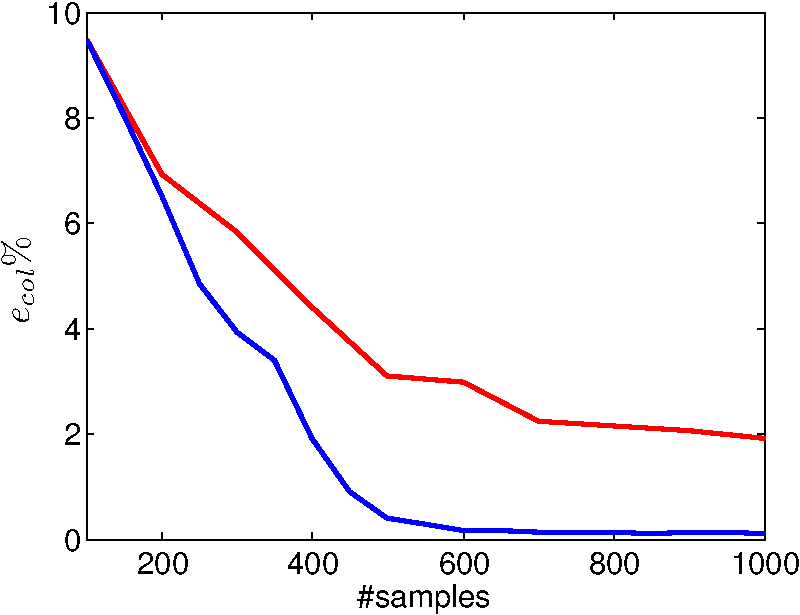
\includegraphics[clip=true, width=0.43\textwidth]{figs/2/active/spider_activelearning-crop.pdf}}
\subfloat[$e_{\text{col}}$ for 3D cup-spoon]{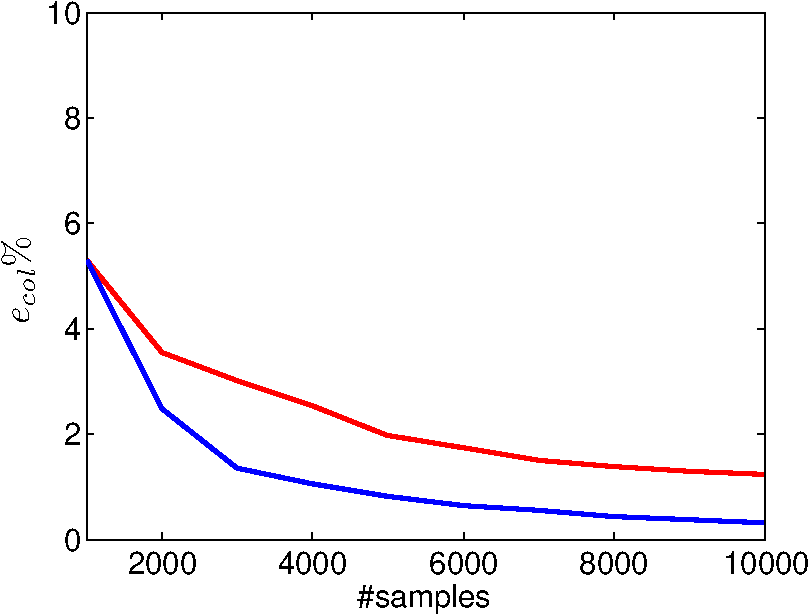
\includegraphics[clip=true, width=0.43\textwidth]{figs/2/active/cupspoon_activelearning-crop.pdf}}
\end{center}
\caption[Relative error convergence of active learning vs. uniform sampling for 2D and 3D object pairs]{Relative error convergence of active learning (blue) vs. uniform sampling (red) for 2D and 3D object pairs. These results demonstrate the benefits of active learning in terms of requiring fewer samples and improved accuracy.}
\label{fig:2:activelearningtime}
\end{figure}

\subsection{Benefits of Active Learning}
A key component of our algorithm is the computation of $\LCS$ by generating appropriate samples in the configuration space. The simplest choice is to perform uniform sampling in $\Cobs (BV(A),BV(B))$ or to use some other random sampling scheme. Instead, we use a combination of active and incremental learning techniques to refine $\LCSi$ and improve its accuracy.


The time and space complexity of the $\LCS$ precomputation phase is a function of
the number of samples used for active learning iterations. The number of samples required to achieve a given error bound $e_{\text{col}}$ depends on both the active learning technique and the underlying classification method used within active learning iterations. It is non-trivial to derive a tight bound on the number of samples required for a specific combination of active learning and classification algorithms. However, we use general results on the sample complexity of active learning~\cite{Hanneke:2013} to show the benefits of our approach.
\begin{theorem}
\label{thm:2:activelearning}
If the number of samples used in active learning iterations of $\LCS$ computation is more than $N$,
where $N=\mathcal O(\log(1/(\epsilon \delta))$, then there exists one active learning technique which can guarantee that with probability at least $1-\delta$, the expected error of the $\LCS$ result will satisfy the bound $e_{\text{col}}\leq\epsilon$.
\end{theorem}

Intuitively, this theorem states there exists a particular active learning technique that will achieve a given bound on $\LCS$ approximation error with high probability.
A proof of this theorem can be obtained based on the CAL (Cohn-Atlas-Ladner) algorithm~\cite{Cohn:ML:1994}. Our $\LCS$ computation is guaranteed to satisfy a bounded error with high probability, if more than $N=\mathcal O(\log(1/(\epsilon \delta))$ samples are used. However, the CAL active learning algorithm is not practical~\cite{Hanneke:2013} and rather we use a combination of exploration and exploitation for active learning (Section~\ref{sec:2:offline:activelearning}) in our $\LCS$ computation algorithm.

Many applications use exploration and exploitation for active learning algorithms. We expect that the use of exploration and exploitation likely also results in a bound similar to Theorem~\ref{thm:2:activelearning}, although the exact derivation of such a bound is a good topic for future research.

Since $e_{\text{col}}$ and $e_{\text{PD}}$ are closely related to each other, Theorem~\ref{thm:2:activelearning} also implies that
$e_{\text{PD}}$ decreases exponentially with the number of samples.
In contrast, when using a uniform sampling strategy to learn the contact space, 
$\LCS$ converges to the
exact contact space
at a polynomial rate as the number of samples
increases~\cite{Mohri:2012:FML}:
\begin{theorem}
\label{thm:2:uniform}
When using uniform sampling, if the number of samples is more than $N$, where $N = \mathcal O(
\frac{1}{2\epsilon^2} \log(2/\delta))$, then
with probability $\geq 1- \delta$, we have the error bound $e_{\text{col}} \leq
\epsilon$.
\end{theorem}

We also measured the expected errors, $e_{\text{col}}$ and $e_{\text{PD}}$, in
complex 2D and 3D benchmarks, as shown in Figure~\ref{fig:2:activelearningtime}.
This demonstrates the high convergence rate and lower error in $\LCS$ computation and PD computation using active learning given the same number
of samples.

\subsection{Benefits of Local Refinement}
Our contact space and PD computation approaches are probabilistic algorithms. Their accuracy is determined by
the samples chosen during the learning phase, including the initial samples and active learning as well as
the runtime queries. As more PD queries are performed within a subspace or a specific region of $\Cspace$,
the accuracy of $\LCS$ in that subspace or region tends to become higher.
This is due to the local refinement step that is performed during runtime whenever we encounter an
inconsistent query configuration.
The incremental learning algorithm updates $\LCS$ around the query configuration by taking into account
local information in $\Cspace$.
In many applications, including dynamic simulation, haptics, or motion planning, a high proportion of
sample queries correspond to positions near the two objects $A$ and $B$. As a result, the runtime
query configurations are relatively close to each other in $\Cspace$ and the local refinement
step improves the accuracy of $\LCS$ in that region. This implies that as more queries are performed in
a localized region of $\Cspace$, the accuracy of $\LCS$ and PD queries improves.
Our algorithm does not make any assumptions about the application or the distribution of runtime query
configurations. We expect that the accuracy of local refinement will improve at the rate given by
uniform sampling (i.e., Theorem~\ref{thm:2:uniform}), rather than at the exponential rate of active learning.
In other words, after generating $N = \mathcal O(1/\epsilon^2)$ samples within a subspace at runtime,
the expected error locally around those samples should be less than $\epsilon$.


\subsection{Time and Space Complexity}
\label{sec:2:analysis:timespacecomplexity}
The precomputation or learning phase is performed for each object pair $(A, B)$
in the environment. The exact collision check is performed using precomputed bounding volume hierarchies.
Given two objects represented as meshes with $m$ and $n$ triangles, the expected cost of a single
exact collision query is $T_{col} = O(\log m + \log n)$.

\begin{figure}[htb]
\begin{center}
\subfloat[$\LCS_0, |S| = 88$]{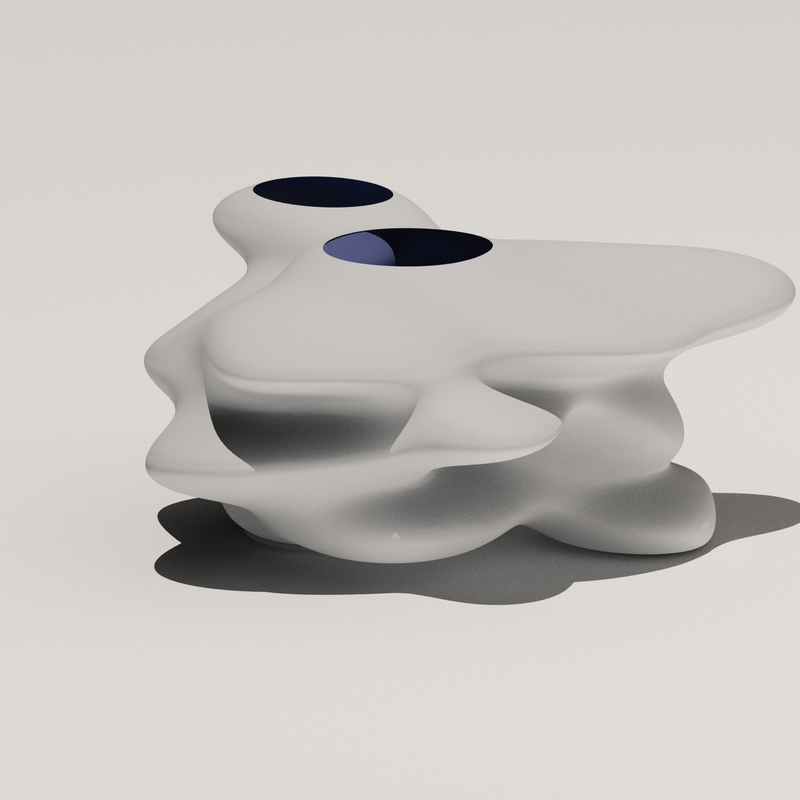
\includegraphics[width=0.24\linewidth]{./figs/2/LCSPDg2D_StarRoom/LCS0.png}}
\subfloat[$\LCS_5, |S| = 174$]{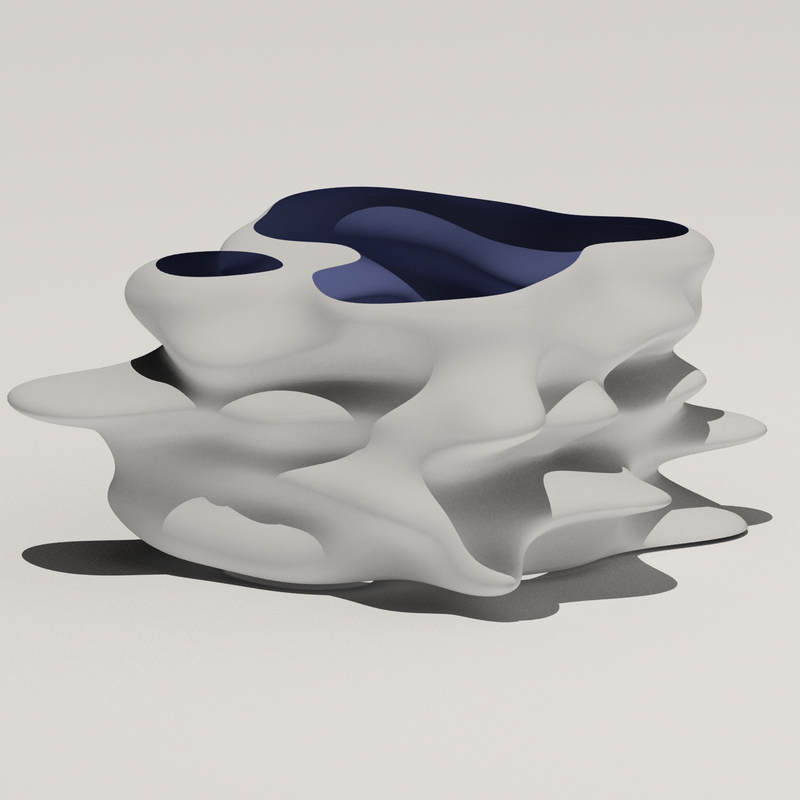
\includegraphics[width=0.24\linewidth]{./figs/2/LCSPDg2D_StarRoom/LCS5.png}}
\subfloat[$\LCS_9, |S| = 237$]{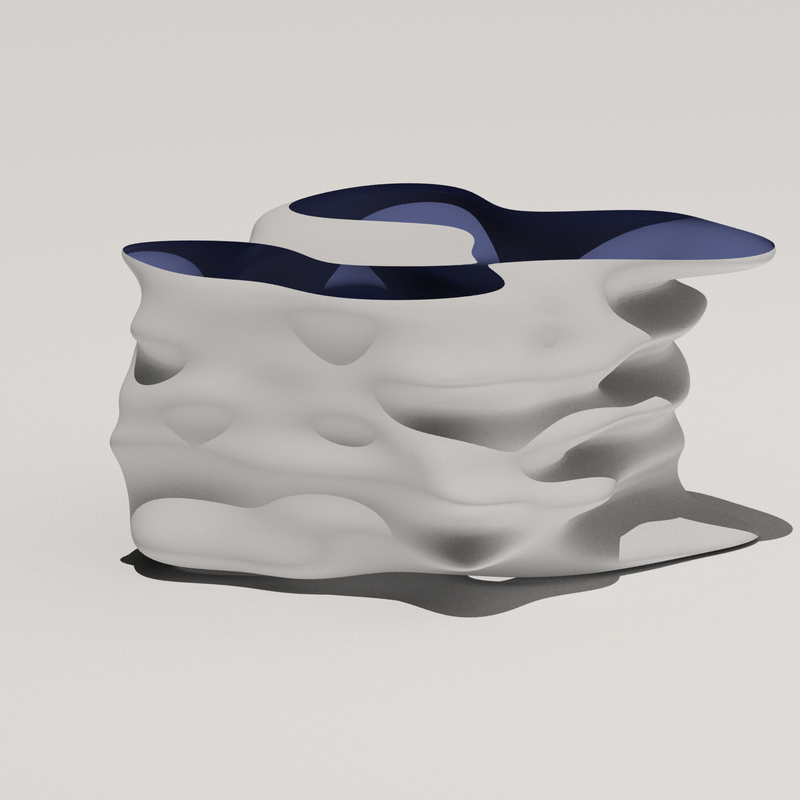
\includegraphics[width=0.24\linewidth]{./figs/2/LCSPDg2D_StarRoom/LCS9.png}}
\subfloat[$\LCS_{12}, |S| = 248$]{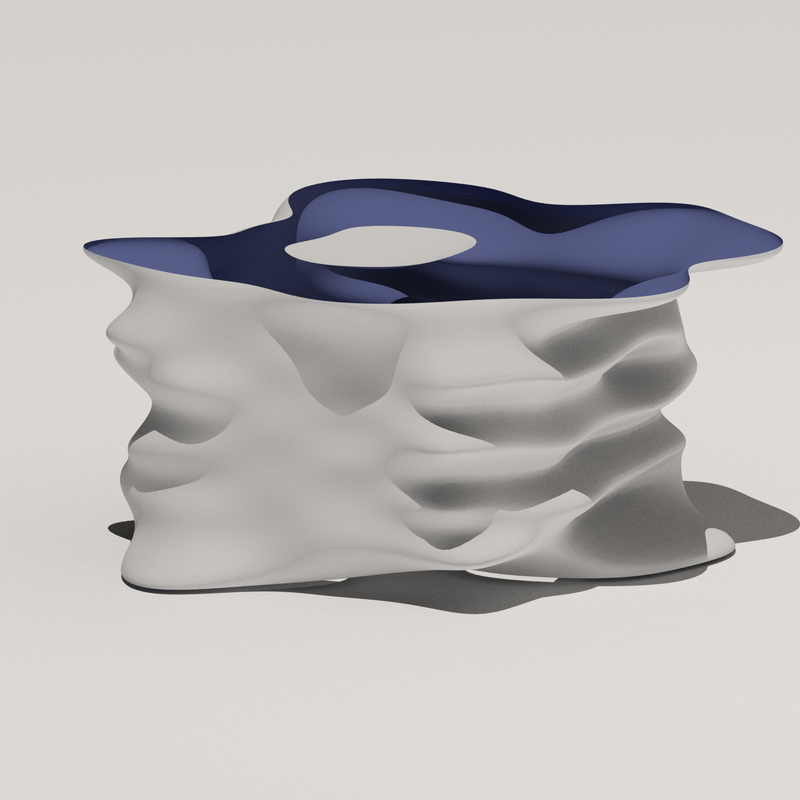
\includegraphics[width=0.24\linewidth]{./figs/2/LCSPDg2D_StarRoom/LCS18.png}}
\caption[$\LCS$ computation using active learning for $\PDg$ query between 2D non-convex shapes]{$\LCS$ computation using active learning for $\PDg$ query between 2D non-convex shapes given in Figure~\ref{fig:2:pipeline}. We show the approximation after $i$-th iteration and the number of support vectors. The vertical axis represents the rotational component of the $\Cspace$. }
\label{fig:2:LCSinActiveLearning2D2}
\end{center}
\end{figure}

\begin{figure}[htb]
\begin{center}
\subfloat[$\LCS_0, |S|=231$]{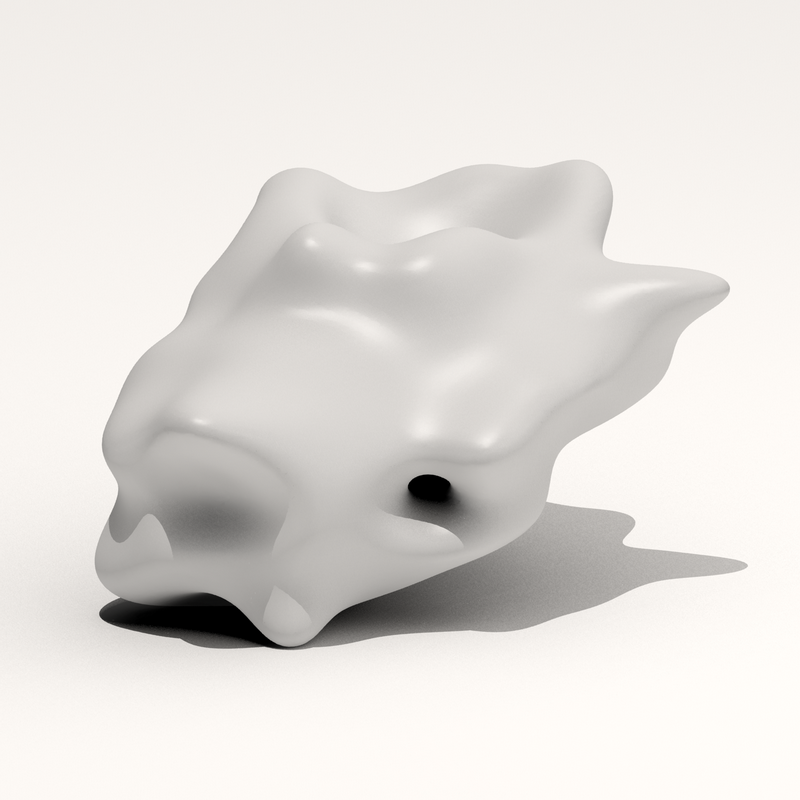
\includegraphics[width=0.24\linewidth]{./figs/2/LCSPDt3D_CupSpoon/LCS0.png}}
\subfloat[$\LCS_5, |S|=869$]{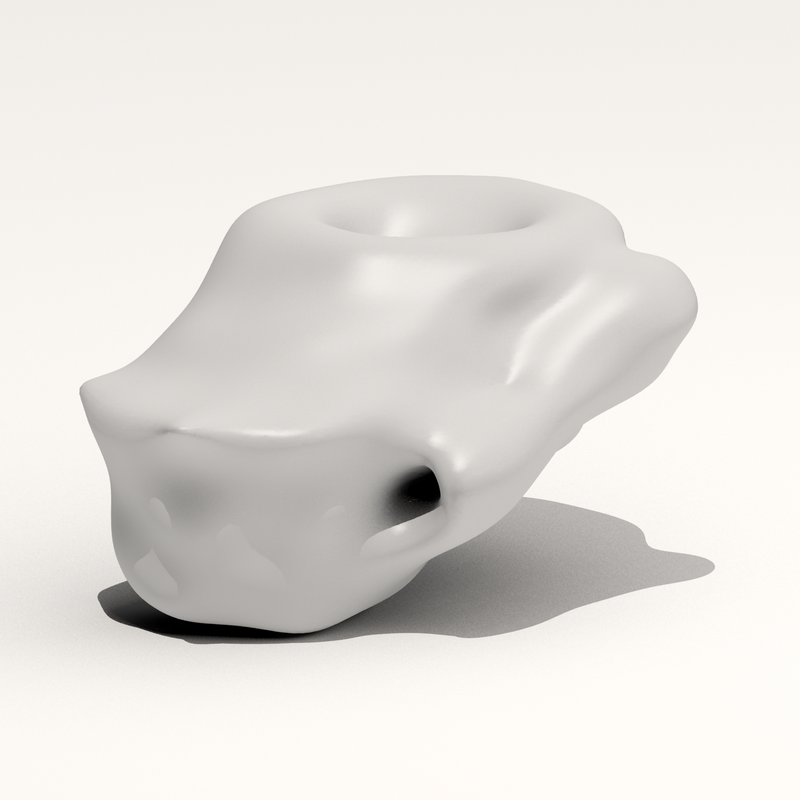
\includegraphics[width=0.24\linewidth]{./figs/2/LCSPDt3D_CupSpoon/LCS5.png}}
\subfloat[$\LCS_9, |S|=1350$]{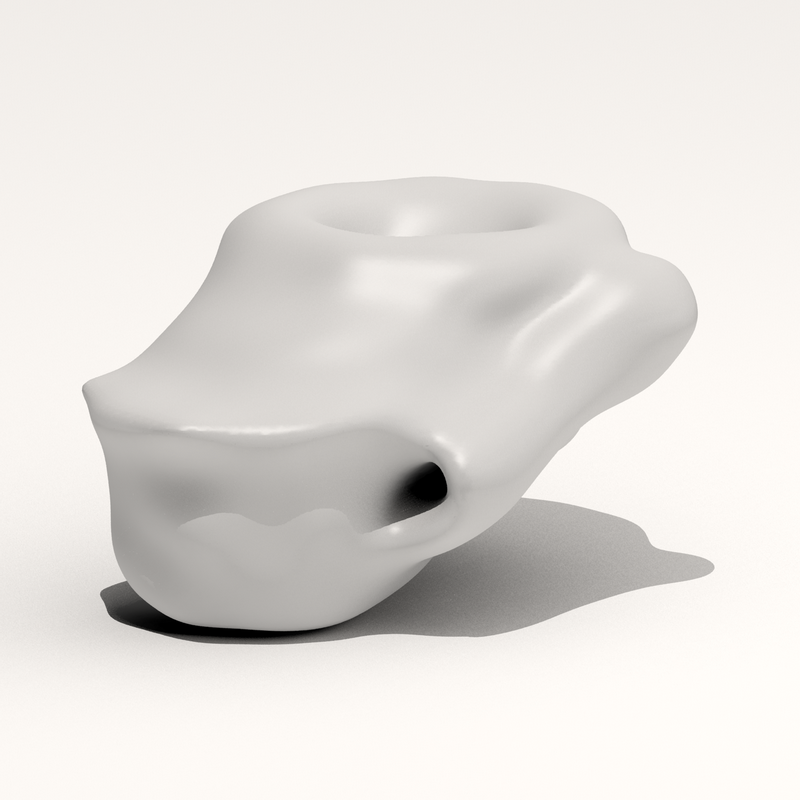
\includegraphics[width=0.24\linewidth]{./figs/2/LCSPDt3D_CupSpoon/LCS10.png}}
\subfloat[$\LCS_{12}, |S|=1572$]{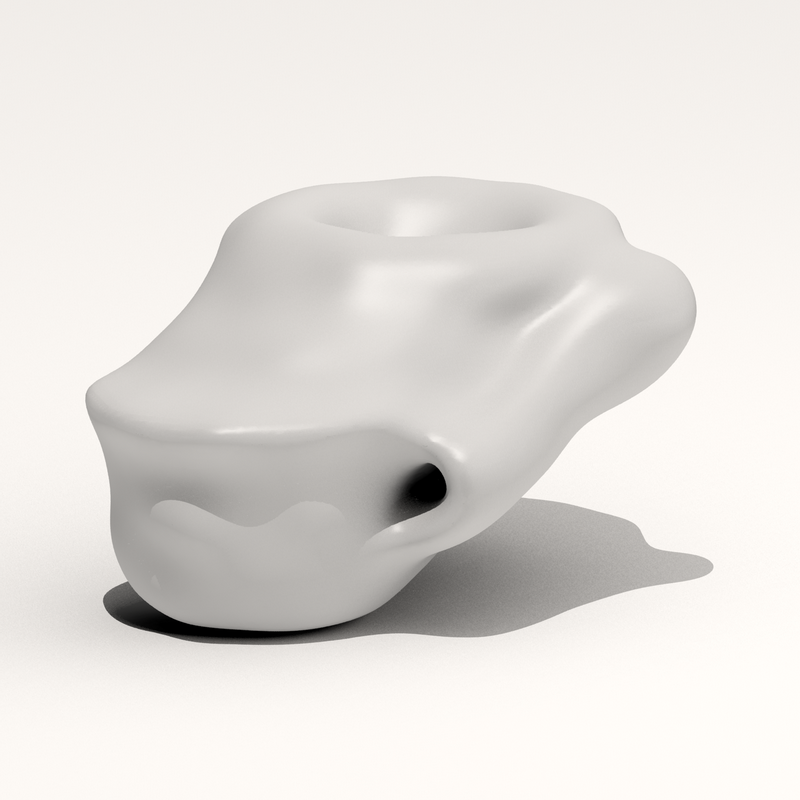
\includegraphics[width=0.24\linewidth]{./figs/2/LCSPDt3D_CupSpoon/LCS17.png}}
\caption[$\LCS$ computation using active learning for $\PDt$ query between 3D cup and spoon]{$\LCS$ computation using active learning for $\PDt$ query between 3D cup and spoon. We provide the number of support vectors corresponding to $\LCSi$. As shown, the algorithm can compute a good approximation in a few iterations.}
\label{fig:2:LCSinActiveLearning3D}
\end{center}
\end{figure}


\paragraph{Offline Learning:} The time complexity for the learning
phase can be estimated as
\begin{align} \label{eq:2:cost}
(T_{LCS_0} + \sum_{i=1}^{I_{AL}} (T_{ES_i} + T_{LCS_i})) + T_{col} \cdot \sum_{i=1}^{I_{AL}} N_{LCS_i},
\end{align}
where $T_{LCS_0}$ is the time complexity to learn the initial approximation;
$T_{ES_i}$ is the time cost to perform exploitation sampling or
exploration sampling in the $i$-th iteration of active learning;
$T_{LCS_i}$ is the time cost for the $i$-th step of incremental
learning, and $I_{AL}$ is the number of iterations performed during active
learning. We denote the number of new samples generated
during $LCS_i$ as $N_{LCS_i}$. We perform collision checking for each sample generated during the learning phase; hence the collision cost is
$T_{col} \cdot \sum_i N_{LCS_i}$.

$T_{LCS_0}$ complexity is governed by the SVM classifier. SVM computation boils down
to solving a constrained quadratic optimization problem using the interior
point or conjugate gradient method, and its worst-case complexity
is $\mathcal O(N_{LCS_0}^{2.3})$.

Incremental learning combines each new sample into $\LCS$ in
constant time, and hence we have $T_{LCS_i} = \mathcal
O(N_{LCS_i})$. $T_{ES_i}$ is the time cost for exploitation sampling
or exploration sampling. For exploration, $T_{ES_i} = \mathcal
O(N_{LCS_i})$. The time complexity for exploitation sampling is
$\mathcal O(|S_{LCS_i}|)$ as we perform interpolation between each
support vector of $\LCSi$ and its $k$-nearest neighbors, which can
be bounded from above as $\mathcal O(\sum_i N_{LCS_i})$.

Overall, the time complexity for the learning phase is
$\mathcal O(\log(\frac{1}{\epsilon}) \sum_i{N_{LCS_i}} +
N_{LCS_0}^{2.3}) + T_{col} \cdot \sum_i N_{LCS_i}$.
The space complexity of our algorithm is linear in the
number of samples used during the learning and runtime phases, and is linear in the number of support vectors in the final $\LCS$ representation.

\paragraph{Runtime Query:} The time complexity in the runtime query
phase depends on $\left| S_{LCS} \right|$, i.e., the number of
support vectors in $\LCS$. $\left| S_{LCS} \right|$ depends on
the smoothness of the exact $\Ccont$, and not as much on the geometric complexity of $A$ and $B$ (see Figures~\ref{fig:2:LCSinActiveLearning2D2} and~\ref{fig:2:LCSinActiveLearning3D}).
For example, the $\Ccont$ of a sphere and another object (i.e., the offset surface) is always smooth, and
therefore a small $\SVLCS$ is sufficient to generate a good approximation of $\Ccont$.
We also notice this in our benchmarks, where $|S|$ for the teeth model (40K triangles) is comparable or higher than that for the bunny (70K triangles), dragon (230K triangles), and Buddha (1M triangles) models. Furthermore, we generated different low-polygon count representations of the Buddha models and observed similar performance on all these approximations.
Thus, the size of
$\SVLCS$ depends on the combinatorial complexity of $\Ccont$ and is also controlled by the tradeoff between 
between the accuracy of PD
computation and the query efficiency.



\section{Implementation and Performance}
\label{sec:2:result}
In this section, we evaluate the performance of our algorithm on complex benchmarks and compare it with prior techniques.
We implemented our algorithm using C++ under Visual Studio 2010
and Windows 7. The two main routines required during the learning phase are exact collision checking between polygonal models and computing the approximate $\LCS$ using support vector machines. At runtime, we need to perform a nearest-neighbor query in the configuration space and to compute a projection using constrained optimization. We used the OBBTree algorithm~\cite{Gottschalk:1996:OHS} for exact collision detection between polygonal objects. We also used a variant of the GJK algorithm~\cite{Gino:2001:GDC} to compute translational penetration depth between convex polytopes, to compare against the performance of our method. In our implementation, we set $\epsilon=2.5\%$ and $\delta=0.01$.

\subsection{Benchmarks}
We have used many complex benchmarks (Figure~\ref{fig:2:demo}) to evaluate the performance of our algorithm. In the simulation, there are multiple contacts between the overlapping objects and we compute $\PDt$ and $\PDg$ between them. The performance of the learning and runtime phases are shown in Table~\ref{tab:2:learningperformance}.

For collision detection, we precompute the BVH for each object, which has a linear memory complexity. For each type of object pair, we precompute the $\LCS$, which takes about 5KB (star-box) to 110KB (teeth, dragon, bunny, Buddha) memory.





\subsection{Physically-based Simulation using PD}
Penetration depth has been used in many dynamic simulators to compute collision response based on penalty forces or constraint-based solvers.
We have integrated our new PD algorithm into two well-known game physics
engines: Box2D~\cite{Erin:2012:Box2D} and Bullet~\cite{Erwin:2012:Bullet}. These engines have support for PD computation based on
convex decomposition and can compute the local translational penetration depth between convex polytopes~\cite{Gino:2001:GDC}.
However, convex decomposition can result in a high number of convex pieces, Moreover, the decomposition-based approach is mainly limited to closed
objects and does not guarantee that two
overlapping non-convex objects will separate, as they only compute local PD using the convex pairs.

\textbf{Contact Points and Normals:} For an inter-penetration configuration $\qa$ and its resulting contact configuration $\qc$, the contact points and contact normal can be computed in the workspace for two objects. First, for the contact configuration $\qc$, its nearest collision-free configuration can be computed using support vectors based on k-nearest-neighbor search in $\Cspace$. Next, the closest points and normals of the given two objects can be computed using the proximity query algorithm~\cite{LGLM00}. Reliable multiple contact points can be obtained using perturbation and persistent contact caching techniques~\cite{Erwin:2012:Bullet}.

\textbf{Box2D} uses PD computation in the impulse-based collision response algorithm.
We demonstrate the performance of our algorithm on
two complex benchmarks (Figure~\ref{fig:2:demo}): (1) angry bird characters falling into a complex chute and (2) Nazca spiders rolling in a tumbler. We precompute the $\LCS$ approximation for a 3-DOF $\Cspace$.
The convex decomposition results in $17$, $30$, and $32$ convex pieces for the BigRedBird, WhiteBird and GreenPig models, respectively. The Nazca spider is decomposed into $77$ convex pieces. We observed an improvement in PD querying of nearly a factor of $20$ when using our active learning algorithm, compared to
techniques based on convex decomposition used in Box2D (see Figure~\ref{fig:2:performancecomparison}(a)(b)). The collision response algorithm is based on the Box2D implementation.


\textbf{Bullet} uses PD computation to handle penetrations in their constraint-based solver.
We demonstrate the benefits of our PD computation algorithm in three scenarios (shown in Figure~\ref{fig:2:demo}):
(1) interlocking $10$ rings; (2) a rainfall of $1,000$ rings; and (3) collapse of a tower composed of $5,500$ rings.
Each ring consists of $256$ triangles and is decomposed into $16$ convex pieces for convex-decomposition.
We precompute the $\LCS$ approximation for a 6-DOF $\Cspace$ and use the approximate result to perform PD queries during the simulation.
Compared to the convex decomposition based algorithm used in Bullet, our PD computation algorithm is about
an order of magnitude faster. We use the standard implementation of contact normal and collision response forces computation available in Bullet.

\textbf{Complex 3D Models}:
We evaluated the performance of our algorithm on many complex models corresponding to the cup-spoon, moving teeth, bunnies, dragons, and Buddha models (Figure~\ref{fig:2:demo}) where we performed $\LCS$ computation for the 6-D $\Cspace$. We observed more than an order of magnitude performance improvement compared to prior methods.


\begin{figure}[t]
  \centering
  \subfloat[$\PDg$: cup-spoon]{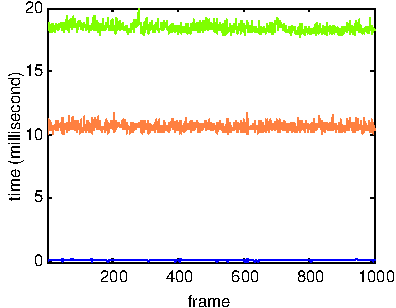
\includegraphics[width=0.49\linewidth]{figs/2/comparison/cupspoon-crop.pdf}}  \hspace{0.05em}
  \subfloat[$\PDg$: rings (Bullet)]{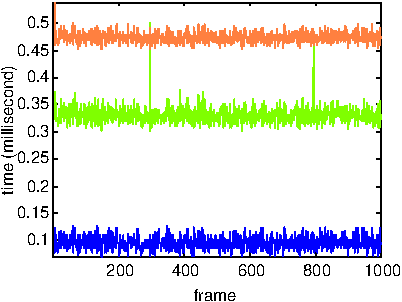
\includegraphics[width=0.49\linewidth]{figs/2/comparison/ring-crop.pdf}}
  \caption[Relative performance of PD computation for different benchmarks]{Relative performance of PD computation for different benchmarks: The blue curve represents the query time computed by our approximate $\PDg$ algorithm. The green curve corresponds to the query time computed using convex decomposition and local PD between convex pairs. The orange curve represents the $\PDg$ query time computed using point-based approximation~\protect\cite{Lien:2009:ASM}.}\label{fig:2:performancecomparison}
\end{figure}





\begin{figure}[htb]
  \centering
  \subfloat[]{\includegraphics[width=0.49\linewidth, page=4]{figs/2/comparison/PD_bunny_bunny.pdf}}
  \subfloat[]{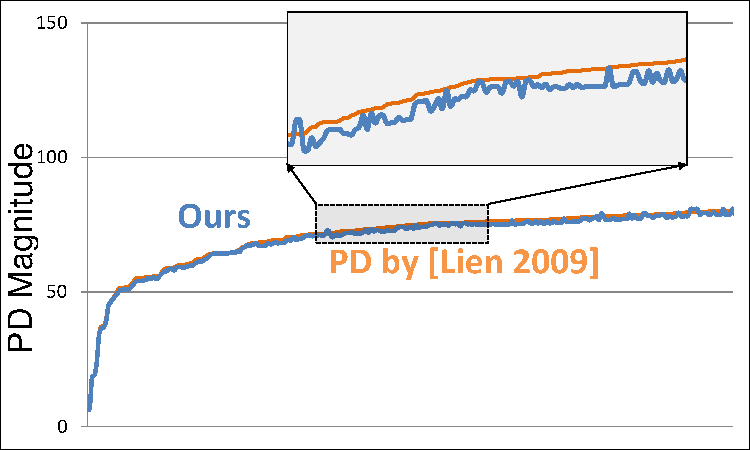
\includegraphics[width=0.49\linewidth, page=1]{figs/2/comparison/PD_bunny_bunny.pdf}}\\
  \subfloat[]{\includegraphics[width=0.49\linewidth, page=2]{figs/2/comparison/PD_bunny_bunny.pdf}}
  \subfloat[]{\includegraphics[width=0.49\linewidth, page=3]{figs/2/comparison/PD_bunny_bunny.pdf}}
  \caption[The performance and accuracy compared to PolyDepth on bunny-bunny benchmark]{The performance and accuracy compared to PolyDepth~\protect\cite{Je:2012:PRP} on the bunny-bunny benchmark. (a) computational time (on average, 0.10ms based on our algorithm vs. 7.15ms in PolyDepth); (b) accuracy comparison between our interactive algorithm vs. an offline algorithm based on Minkowski sum~\protect\cite{Lien:2009:ASM}; (c) accuracy comparison of PD computation between our algorithm vs. PolyDepth; (d) our global PD algorithm (blue) has lower error compared to PolyDepth, which performs local optimization. }\label{fig:2:bunnymodels}
\end{figure}

\begin{figure}[htb]
  \centering
  \subfloat[]{\includegraphics[width=0.49\linewidth, page=4]{figs/2/comparison/PD_dragon_dragon.pdf}}
  \subfloat[]{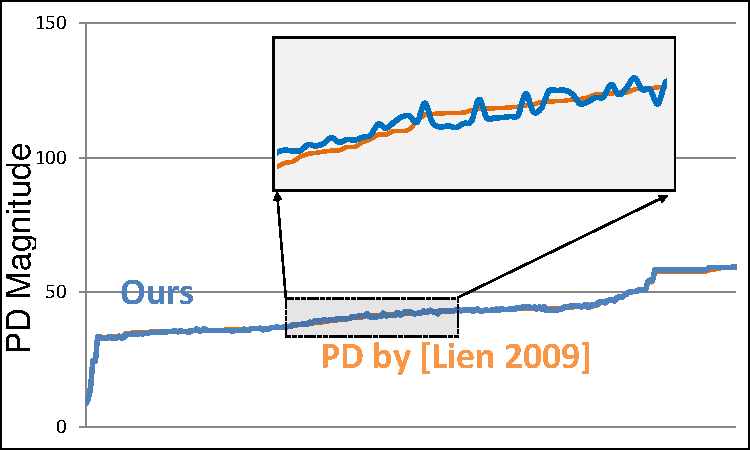
\includegraphics[width=0.49\linewidth, page=1]{figs/2/comparison/PD_dragon_dragon.pdf}}\\
  \subfloat[]{\includegraphics[width=0.49\linewidth, page=2]{figs/2/comparison/PD_dragon_dragon.pdf}}
  \subfloat[]{\includegraphics[width=0.49\linewidth, page=3]{figs/2/comparison/PD_dragon_dragon.pdf}}
  \caption[The performance and accuracy compared to PolyDepth on dragon-dragon benchmark]{The performance and accuracy compared to PolyDepth~\protect\cite{Je:2012:PRP} on the dragon-dragon benchmark. (a) computational time (on average, 0.12ms based on our algorithm vs. 9.86ms in PolyDepth); (b) accuracy comparison between our interactive algorithm vs. an offline algorithm based on Minkowski sum~\protect\cite{Lien:2009:ASM}; (c) accuracy comparison of PD computation between our algorithm vs. PolyDepth; (d) our global PD algorithm (blue) has lower error compared to PolyDepth, which performs local optimization.}\label{fig:2:dragonmodels}
\end{figure}



\subsection{Comparison with Prior Methods}
Most existing practical algorithms perform local analysis of the intersection regions and
compute local PD. Other techniques use distance fields and can be accelerated using GPUs. In practice, these techniques are quite fast and can also handle
deformable models. On the other hand, our global PD algorithm involves preprocessing and is mainly designed for rigid objects.
The performance of our runtime query (e.g., about $0.1\sim2$ milliseconds) is comparable to or faster than these local PD computation algorithms. The main benefit of our approach over local PD methods is the computation of global
translational and rotational PD, which provides a more reliable measure of separating two overlapping objects.
Other algorithms reduce PD computation to constrained optimization~\cite{Nawratil:2009:GPD,Zhang:2007:AFP,Je:2012:PRP}.
In these techniques, a sequence of configuration samples on the contact space are iteratively
computed until a local minimum configuration is found. The
performance of these algorithms heavily relies on the initial guess of the configuration, and it is hard to provide
error bounds in terms of global PD (see Figure~\ref{fig:2:bunnymodels} and~\ref{fig:2:dragonmodels}). The approximate PD computed by our global algorithm can be used as an initial guess for these optimization-based techniques and thereby improve their accuracy.


In order to evaluate the error in our approximate PD computation algorithm, we compute very accurate PD between two objects. For translational PD, the exact PD can be obtained by computing the Minkowski sum between two objects. 
It is difficult to compute exact Minkowski sum for complex 3D objects like the teeth or dragon, due to the combinatorial complexity arises. Instead we use the point-based algorithm~\cite{Lien:2009:ASM} to approximate the PD and estimate the error of our algorithm.
For generalized PD, the exact PD computation is even harder. Therefore, we approximate the exact contact space with many slices of Minkowski sums. Intuitively, we sample many rotations in rotation space and then compute Minkowski sums for all the rotations. The combination of these Minkowski sums is used as an approximation of the contact space. We label the PD computed using these offline techniques as "\emph{nearly exact PD}" for our algorithm and comparisons.
In practice, our approach is more than an order of magnitude faster than other algorithms that are based on convex decomposition (e.g., \cite{Kim:2002:FPD} for $\PDt$; \cite{Zhang:2007:GPD} for $\PDg$) or point-based approximations. We have compared the runtime performance of our algorithm with these prior global methods in Figure~\ref{fig:2:performancecomparison}. More benchmarks, results, and comparisons are given in the supplementary material.


\section{Limitations}
Our approach is the first attempt at using machine learning techniques to improve the peformance and quality of penetration-depth computation. In order to make this method useful for real-world applications, we need to solve some important limitations. In our discussion, we divide these limitations into two categories: limitations related with approximate configuration space computation, and limitations related with approximate penetration-depth computation.

\subsection{Limitations Related with Approximate Configuration Space Computation}
The first limitation related with approximate configuration space computation is that the precomputation phase must be performed for each pair of moving objects in the simulation. Thus, in the worst case, its complexity grows as a quadratic function of the number of objects in the simulation. In addition, the accuracy and running time of our learning phase is a function of the combinatorial complexity of the contact
space and the sampling scheme. Hence, it is possible that our method may not generate a sufficient number of samples in small,
isolated components of contact space, or it may take a large number of iterations.
Moreover, the overall approach is probabilistic, and all of our error bounds are derived in terms of expected error.

\subsubsection{Failure in Extreme Cases}
In Section~\ref{sec:2:intro}, we claimed that our method is general and is able to compute the contact space for complex non-convex and non-manifold models. However, this claim is based on the implicit assumption that a `correct' collision detection routine is available for input geometric data; the `correctness' means that the collision result provided by the collision checking routine can correctly reflect the objects' collision status in physical world. Whether the above assumption holds will determine the correctness of the contact space computed by our learning framework. For example, if objects are represented as meshes, the assumption generally holds even if input meshes are non-convex, non-manifold, or not-closed, so our method usually can return a correct approximate contact space. However, the assumption may not hold for meshes in several extreme cases. First, if two objects are so different in scale that one object $A$ can be completely contained inside the other object $B$, the mesh-mesh collision checking will always report collision-free for configurations in which $A$ locates inside $B$, while in physical world $A$ and $B$ should be in-collision. Thus, our learning framework will not provide a correct contact space in this case. Second, if the mesh representation of object $B$ has a hole larger than the size of object $A$, the collision checking will also give incorrect results and our learning framework will fail to compute a reasonable contact space. There are several possible solutions to this limitation, including 1) designing better collision checking routines for these extreme cases; and 2) using the solid geometry instead of meshes to represent objects.

\subsubsection{SVM Implementation}
When describing the learning framework in Section~\ref{sec:2:offline:svm}, we use the hard-margin SVM (Equation~\ref{eq:2:svm1}) to introduce the key-points in the algorithm, since all in-collision samples and collision-free samples are separable. However, in implementation we use the soft-margin SVM defined as follows:
\begin{align}
\label{eq:2:svmsoft}
& \underset{\mathbf w, b, \xi}{\text{min}} & & \frac{1}{2}\|\mathbf w\|^2 + C \sum_{i=1}^k \xi_i & &  \\
& \text{subject to} & & c_i (\mathbf w \cdot \phi(\mathbf q_i) + b)
\geq 1 - \xi_i, & & \xi_i \geq 0 & & 1 \leq i \leq k. \notag
\end{align}
In soft-margin SVM, slack variables $\xi_i$ measure the degree of misclassification of the data; the objective function is increased by a term which uses weight variable $C$ to penalize non-zero $\xi_i$. The optimization becomes a trade-off between a large margin and a small error penalty. 

In practice, a soft-margin SVM behaves better than a hard-margin SVM, even when data is separable as in our case. The reason is that for a hard-margin SVM, a single outlier (e.g., a sample extremely close to the actual contact space) can determine the boundary, which makes the classifier overly sensitive to the data. For contact space learning, a hard-margin SVM will provide a uneven contact space with jagged edges, while the soft-margin SVM can provide a smooth contact space. 

However, the soft-margin SVM requires an appropriate $C$ as the input, which is not an easy task. A suitable value of $C$ is related with the set of samples used to learn a contact space; it is also related with the number of samples used. A too small $C$ will result in a large error in the resulting contact space, while a too large $C$ will result in a non-smooth contact space or a contact space with the incorrect topology. Theoretically, cross-validation provides a systematic manner for choosing $C$, but it is computationally expensive. In our experiment, we simply repeate the learning algorithm several times and choose the $C$ leading to the best result.

\subsubsection{Learning on Non-Manifold Structure}
When learning a contact space in $\SEcubic$, we simply convert every configuration into a vector in Eculidean space: for the rotation component of each configuration, we either convert it into a $3$-dimensional vector for Euler angles or into a $4$-dimensional vector for quaternions. Given the vector representation of each configuration, we then perform the learning algorithm directly in Euclidean space. However, $\SEcubic$ in fact is a Lie group and the Eculidean space approximation is only valid locally around each configuration. Our current method does not consider additional constraints and structures from the underlying Lie group and thus may not provide good results for contact spaces with significant rotation components. One possible solution to fix this limitation is using learning algorithms on Lie group~\cite{Tuzel:2008:LLG}.

\subsection{Limitations Related with Approximate Penetration-depth Computation}

\subsubsection{Penetration-Depth Formulation}

First, the solution to the penetration depth problem is often not unique or differentiable. Since we compute
a bounded-error approximation of PD, there could be multiple solutions that satisfy those error bounds.
This discontinuity in PD formulation and computation can cause instability in collision response for haptic rendering. In complex rigid-body simulations with multiple objects, global PD computation can improve the accuracy of the simulation, but cannot guarantee that it is totally collision-free.

Second, the penetration depth definition used in our method is a pure geometric one. In particular, the penetration-depth is completely determined given two objects and their configurations, and is not related with objects' velocity and acceleration. As a result, the penetration depth value computed by our method does not have physical meaning, and may not be accurate enough for applications like physically-based simulation.

\subsubsection{$\knn$ Metric}
The result of 

Section~\ref{sec:2:overview:pdformulation}

2. metric: given two configuration q1, and q2, compute the relative configuration. q then find the closest qc, but qc * q is closest to q2? if give rotation large weight-->find the rotation closest to query, but the resulting PD is large. If given rotation small weight --> rotation far from query may have small PD.   not trivial. THe PD metric we used: not scale: $I = mr^2 / V = r^2$.


\subsubsection{Noisy PD Values}








3. noisy a) When configuration space average error is small, the PD error usually is small. but error is not distributed uniformly. and PD error is much larger than configuration space error. As PD is analogous to the directive of the C-space.   b) rotation a bit, will have larger error, why? discrete sample

4. to generate a smooth motion, need much more samples than the number of samples required. (show some result)




\section{Conclusions}
We have presented a novel approach for the computation of translational and generalized PD between polygonal models.
The main idea is to sample the configuration space and approximate the contact space based on
machine learning classifiers. We use support vector machines to approximate the contact space, and
the runtime PD query is reduced to nearest neighbor computation. Furthermore,
we use active learning techniques to select the samples when approximating the contact space.
Our overall approach is general and applicable to all polygonal models.
We have demonstrated the interactive performance of our algorithm on complex, non-convex models and have also used
our algorithm for collision response in game physics engines.
To the best of our knowledge, this is the first approach that is able to compute global and reliable PD between rigid models at
interactive rates.


There are many avenues for future work, including overcoming the stated limitations. The basic components of our learning and run-time phases, such as SVM learning, collision detection, and nearest-neighbor computation, can be accelerated using GPU parallelism. We can use other active learning techniques to improve the sampling as well as other classifiers or learning techniques to improve the accuracy or convergence of \LCS. It would also be useful to derive tight theoretical error bounds (e.g., Theorem~1) for active learning algorithms based on exploitation and exploration.
It would also be useful to extend the approach to articulated models that take into account self-collisions between various links.
In order to handle deformable models, we aim to develop incremental techniques that can refine the contact
space approximation for deforming objects. It would be useful to apply this approach for other PD formulations, such as penetration volume~\cite{Weller-RSS-09}, which can result in continuous response forces. We also need improved algorithms for collision response that can guarantee collision-free simulations for interactive applications.

\begin{figure}
\centering
\parbox{0.9\linewidth}{%
 \subfloat[]{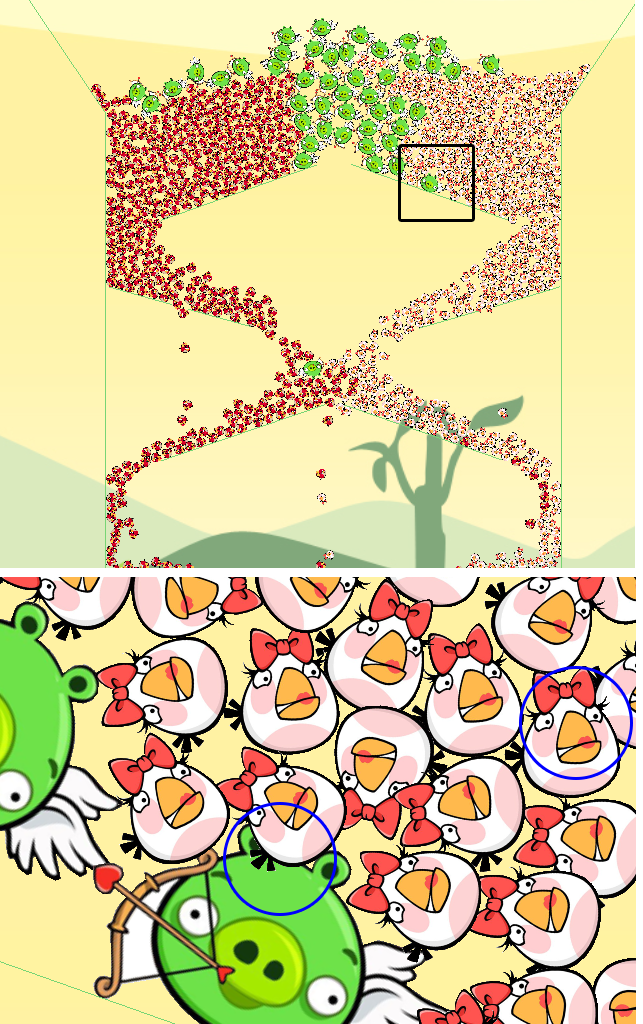
\includegraphics[height=0.605\linewidth]{figs/2/demo/Box2D/Box2DAngryBird_2013_5_14.png}}
 \subfloat[]{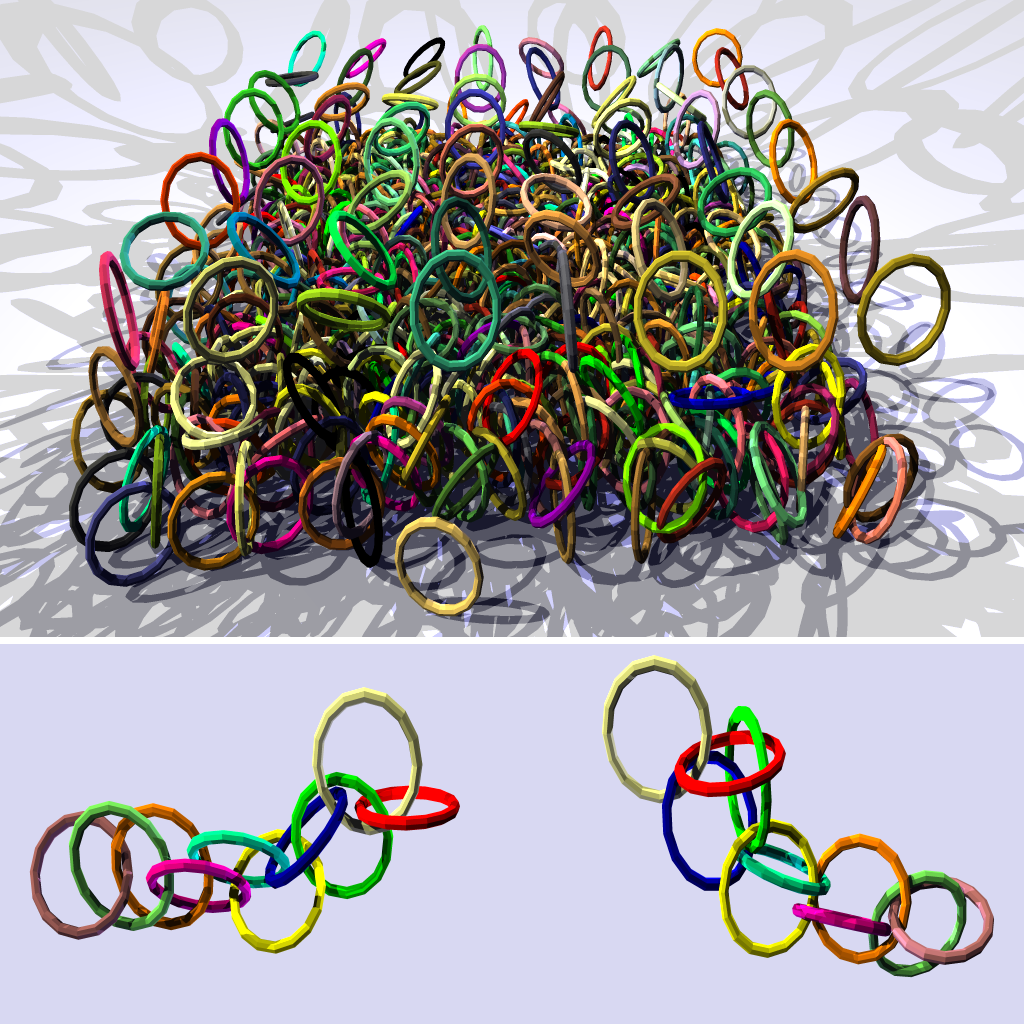
\includegraphics[height=0.605\linewidth]{figs/2/demo/Bullet/BulletRainfall.png}}
}
\parbox{0.85\linewidth}{%
  \subfloat[]{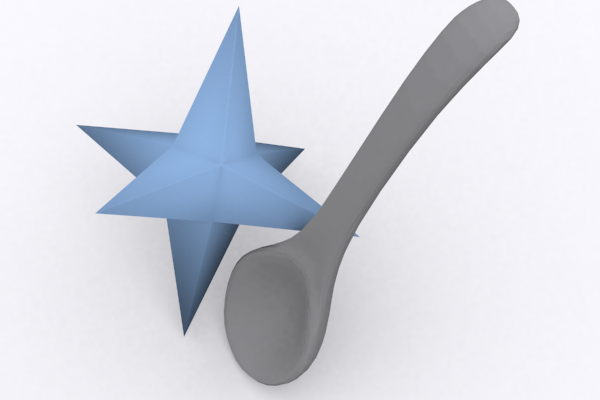
\includegraphics[width=0.325\linewidth]{figs/2/demo/star_spoon.png}}
  \subfloat[]{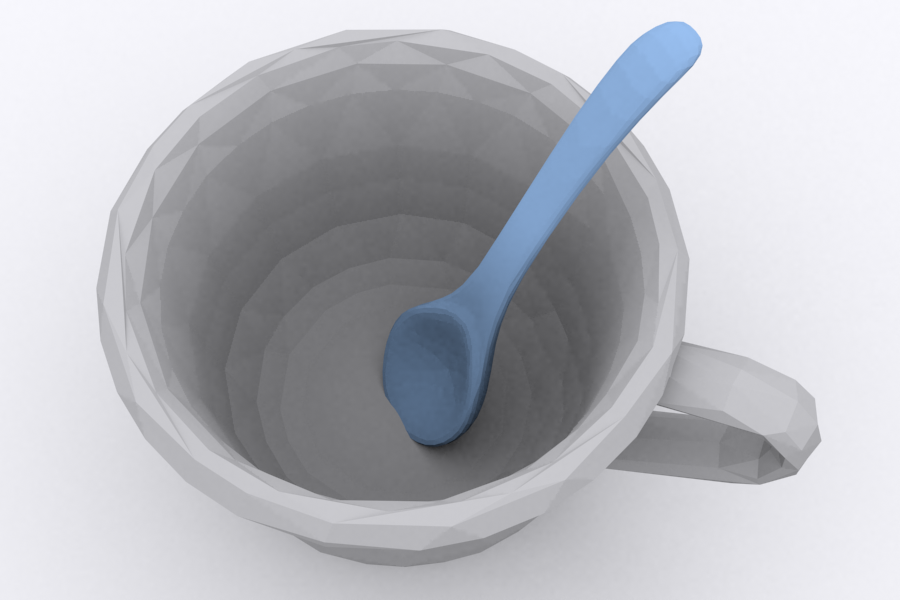
\includegraphics[width=0.325\linewidth]{figs/2/demo/cup_spoon.png}}
  \subfloat[]{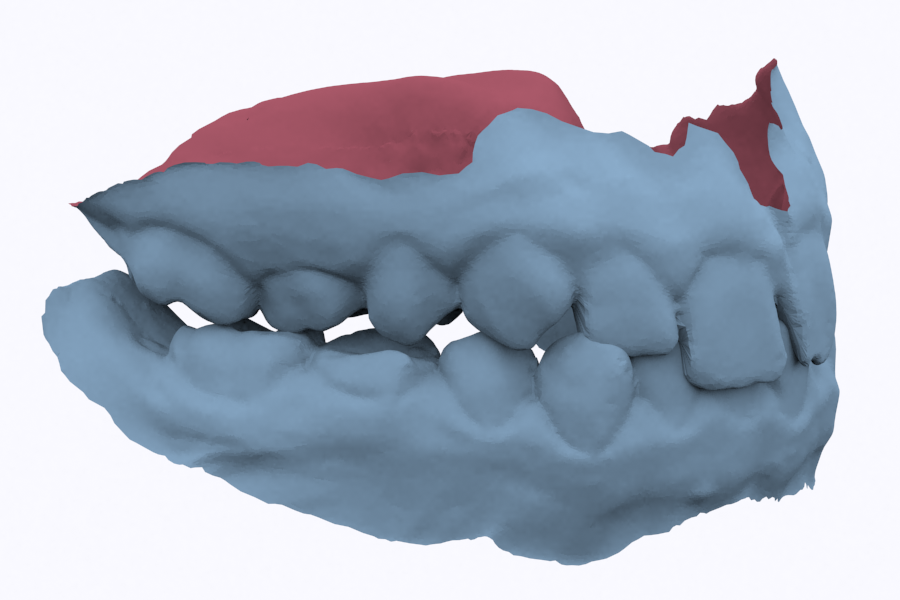
\includegraphics[width=0.325\linewidth]{figs/2/demo/teeth.png}}\\
  \subfloat[]{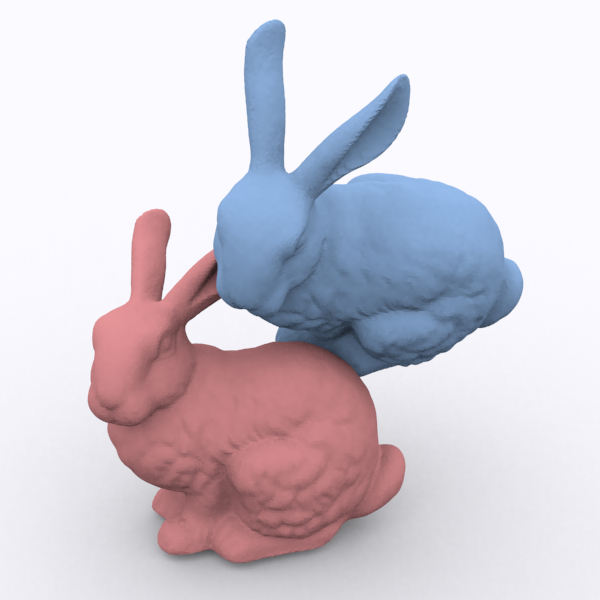
\includegraphics[width=0.325\linewidth]{figs/2/demo/bunny_bunny.png}}
  \subfloat[]{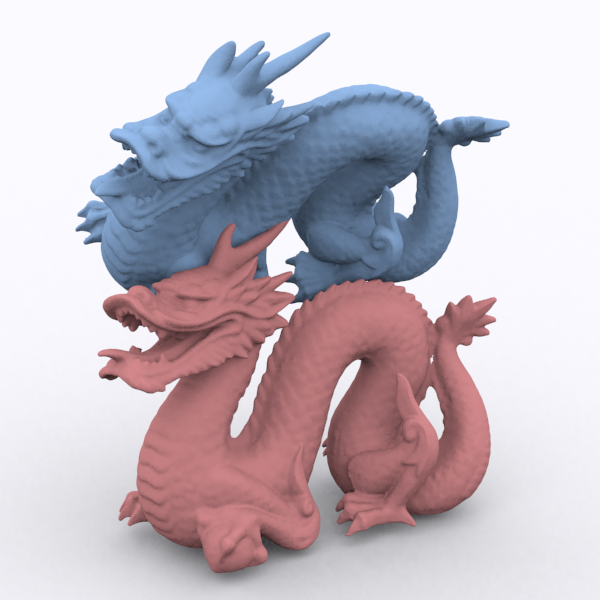
\includegraphics[width=0.325\linewidth]{figs/2/demo/dragon_dragon.png}}
  \subfloat[]{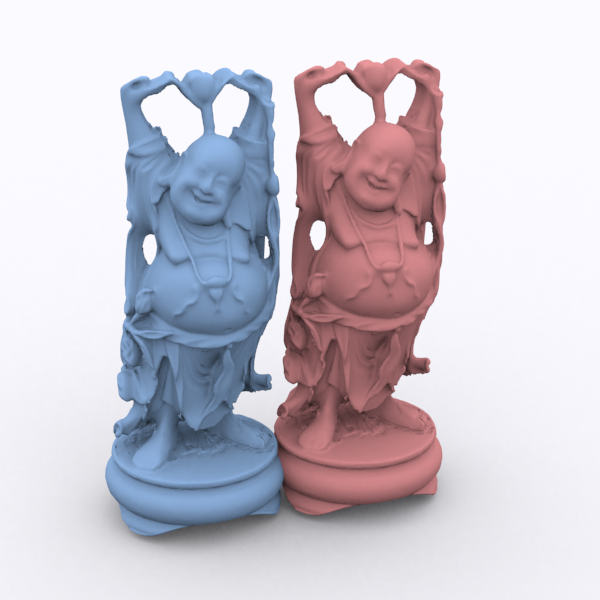
\includegraphics[width=0.325\linewidth]{figs/2/demo/buddha_buddha20K.png}}
}
\caption[Learning-based PD computation algorithm computes a global penetration depth between overlapping non-convex and non-manifold objects]{Our algorithm computes a global penetration depth between overlapping non-convex and non-manifold objects. (a) Dynamic simulation of angry bird characters falling into a complex chute in the Box2D physics engine; (b) rainfall of $1,000$ rings in the Bullet physics engine; (c) a star and a spoon; (d) a spoon and a cup; (e) multiple contacts between upper and lower teeth (each has more than $40,000$ triangles). (f-h) benchmarks consisting of complex models (bunny, dragon and Buddha models have $70K$, $230K$ and $1M$ triangles, respectively). For each pair of overlapping objects, our PD algorithm takes less than $0.1\sim2$ milliseconds, with less than 2-3\% relative error.}\label{fig:2:demo}
\end{figure}


\begin{table}[tbp]
  \centering
  \rowcolors{1}{gray!25}{}
  \resizebox{\linewidth}{!}{%
    \begin{tabular}{|c|r|r|r|r|r|r|r|r|r|r|r|r|r|r|}
    \hline
    \multicolumn{2}{|c|}{\multirow{3}{*}{Model}} & \multicolumn{8}{c|}{Offline Learning  \LCS} & \multicolumn{5}{c|}{Runtime Query}\\
    \cline{3-15}
    \multicolumn{2}{|c|}{} & \multicolumn{2}{c|}{Initial Learning} & \multicolumn{4}{c|}{Active Learning} & \multicolumn{1}{c|}{\multirow{2}{*}{total (s)}} & \multicolumn{1}{c|}{\multirow{2}{*}{mem}} & \multicolumn{4}{c|}{time (ms)} & \multicolumn{1}{c|}{\multirow{2}{*}{$e_{\text{PD}}$(\%)}}\\
    \cline{3-8} \cline{3-8} \cline{11-14}
    \multicolumn{2}{|c|}{} & \#smpls & time (s) & \#smpls & $|S|$ & $e_{\text{col}}$ (\%) & time (s) & \multicolumn{1}{c|}{}& \multicolumn{1}{c|}{}&  NN & projection & refine & total & \multicolumn{1}{c|}{}\\
    \hline \hline
    \multicolumn{1}{|c|}{\multirow{3}{*}{2D $\PDt$}} & star vs. room & 100   & 0.006 & 1000 & 374   & 1.88 & 0.15  & 0.156 &  4.4  & 0.065 & 0.02 & 0.03 & 0.115 & 0.023\\
    \multicolumn{1}{|c|}{} & monkeys & 100   & 0.4   & 1000 & 346   & 0.11 & 2.74  & 3.14 &  4.2  & 0.06 & 0.01 & 0.03   & 0.10 & 0.008 \\
    \multicolumn{1}{|c|}{} & spiders & 100   & 0.01  & 1000 & 389   & 1.37 & 0.27  & 0.28 &  4.7  & 0.066 & 0.01 &  0.02  & 0.096 & 0.025 \\ \hline
    \multicolumn{1}{|c|}{\multirow{3}{*}{3D $\PDt$}} & star vs. spoon & 1000  & 0.08  & 10000 & 1105  & 0.59 & 1.245 &  1.33 &  17  & 0.43 & 0.21 & 0.02  & 0.66 & 0.012\\
    \multicolumn{1}{|c|}{} & cup vs. spoon & 1000  & 0.25  & 10000 & 1472  & 0.75 & 4.46 & 4.81 &   23  & 0.54 & 0.22 &  0.03  & 0.79 & 0.019 \\
    \multicolumn{1}{|c|}{} & rings & 1000  &  0.20 & 10000 & 1224  & 0.56 & 11.99 & 12.01 & 19    & 0.66 & 0.12 &  0.05   &  0.83 & 0.016 \\
    \multicolumn{1}{|c|}{} & teeth  & 1000  &  0.33 & 10000 & 2132  & 1.3 & 43.21 & 43.54 &  34   & 1.3 & 0.2 &  0.08  &  1.58 & N/A \\
    \multicolumn{1}{|c|}{} & bunnies  & 1000  &  0.15 & 10000 & 666  & 1.7 & 36.49 & 36.64 &   11    & 0.1 & 0.12 &  0.04  & 0.26 & 2.0 \\
    \multicolumn{1}{|c|}{} & dragons  & 1000  &  0.17 & 10000 & 854  & 1.8 & 31.11 & 31.28 &   14    & 0.13 & 0.11 &  0.05  &  0.29 & 1.9 \\
    \multicolumn{1}{|c|}{} & Buddha  & 1000  &  1.7 & 10000 & 1384  & 1.8 & 37 & 38 &   22    & 0.18 & 0.10 &  0.09  &  0.37 & 1.8 \\
    \hline \hline
    \multicolumn{1}{|c|}{\multirow{3}{*}{2D $\PDg$}} & star vs. room &  100   & 0.005 & 2000 & 436  & 2.0 & 1.276 & 1.281 &  6.9   & 0.08 & 0.03 &  0.02    & 0.13 & 0.021\\
    \multicolumn{1}{|c|}{} & monkeys & 100 & 0.42   &  2000 & 545   & 0.43 &  5.84 &  6.26 &    8.7    & 0.07 & 0.02  & 0.02  & 0.11 & 0.013 \\
    \multicolumn{1}{|c|}{} & spiders & 100 & 0.011 & 2000   & 540  &  0.8 &  1.16 & 1.17 &   8.6   & 0.08 & 0.02 &   0.01   & 0.11 & 0.018 \\ \hline
    \multicolumn{1}{|c|}{\multirow{3}{*}{3D $\PDg$}} & star vs. spoon &  1000 & 0.095  & 10000  & 1731  & 1.9 & 37.49 & 37.58 &  48   &0.5 & 0.25 &  0.05  & 0.80 & N/A \\
    \multicolumn{1}{|c|}{} & cup vs. spoon & 1000 & 0.3  & 10000   &  2107  & 1.2  &  78.34 & 78.64 &  59   & 0.3& 1.0 & 0.03  &  1.33 & N/A \\
    \multicolumn{1}{|c|}{} & rings & 1000  & 0.25  & 10000   &  1977  &  1.3  &  223.1 & 223.4 &   55    & 0.82 & 0.21 &   0.03  & 1.06 & N/A \\
    \multicolumn{1}{|c|}{} & teeth  & 1000  &  0.54 & 10000 & 3216  & 2.8 & 476.43 & 476.97 &   90      & 2.2 & 0.2 & 0.04  &  2.44 & N/A \\
    \multicolumn{1}{|c|}{} & bunnies  & 1000  &  0.33 & 10000 & 2283  & 3.1 & 342.31 & 342.64 &   64     & 0.89 & 0.12 & 0.02  &  1.03 & N/A \\
    \multicolumn{1}{|c|}{} & dragons  & 1000  &  0.37 & 10000 & 2387  & 2.8 & 378.92 & 477.29 &   69     & 1.01 & 0.18 & 0.03  &  1.22 & N/A \\
    \multicolumn{1}{|c|}{} & Buddha  & 1000  &  2.3 & 10000 & 3765  & 2.7 & 643 & 645 &   105     & 1.20 & 0.28 & 0.07  &  1.55 & N/A \\
    \hline
    \end{tabular}
}
  \caption[Performance of the learning-based PD algorithm on 2D and 3D models]{
Performance of our PD algorithm on 2D and 3D models: The learning phase includes the number of samples, size of support vectors, final memory usage (KB), and precomputation time.
We also give a timing breakdown of runtime queries. The PD error is computed by comparing the accuracy of $\overline{\text{PD}}$ with prior algorithms used for PD computations. For accurate $\PDt$ computation, we use the accurate, offline algorithm of~\protect \cite{Lien:2009:ASM} or use a combination of convex decomposition and Minkowski sums.   Since no accurate and efficient algorithms are known for many PD queries (e.g., $\PDt$ computation for non-closed meshes like teeth model; $\PDg$ computation for 3D models), we do not analyze the accuracy of our algorithm in such cases (shown as N/A). }\label{tab:2:learningperformance}
\end{table}













